% =============================================================================
% 流体力学（水力学）自学讲义 · 第 6 部分
% 第五章 5.3--5.5：沿程与局部水头损失
% 模式：passive-study · 主题：teal · 图示：TikZ 重绘
% =============================================================================
\documentclass[aspectratio=169,10pt]{beamer}
\usepackage[teal]{template-lib/template-lib}
\uselayout{text}\uselayout{eq}\uselayout{twocol}\uselayout{1img}\uselayout{table}
\usetikzlibrary{arrows.meta,calc,positioning,patterns,decorations.pathmorphing,decorations.pathreplacing,decorations.markings}

% ── 记号缩写 ─────────────────────────────────────────────────────────────────
\newcommand{\rd}{\,\mathrm{d}}
\newcommand{\dd}[2]{\frac{\mathrm{d}#1}{\mathrm{d}#2}}
\newcommand{\pd}[2]{\frac{\partial #1}{\partial #2}}
\newcommand{\DDt}[1]{\frac{\mathrm{D}#1}{\mathrm{D}t}}
\newcommand{\grad}{\nabla}
\newcommand{\divg}{\nabla\!\cdot}
\newcommand{\vc}[1]{\boldsymbol{#1}}
\newcommand{\Real}{\mathbb{R}}
\newcommand{\Rey}{\mathit{Re}}
\newcommand{\atm}{\mathrm{atm}}
\newcommand{\proofskipnote}{\footnote{\scriptsize 非数学背景读者：本帧为\emph{推导细节}，第一遍可先跳过，记住本帧\emph{要点}即可。}}

% 本地化模板中的 takeaway 标签。
\renewcommand{\TLtakeaway}[1]{%
  \vspace{0.25em}%
  \begin{tikzpicture}
    \node[fill=TLaccentLight, rounded corners=3pt, inner sep=7pt,
          text width=\dimexpr\linewidth-14pt\relax, align=justify] {%
      \small\textcolor{TLaccent}{\textbf{要点。}} #1%
    };
  \end{tikzpicture}%
  \vspace{0.1em}%
}

\TLsetfoot{流体力学（水力学）\textperiodcentered{} 自学讲义 \textperiodcentered{} 第 6 部分：沿程与局部水头损失}

\begin{document}
\emergencystretch=30em

% =============================================================================
% A. 标题 + 如何使用 + 承前
% =============================================================================
\TLtitlecenter
  {沿程与局部水头损失}
  {流体力学（水力学）自学讲义 \textperiodcentered{} 第 6 部分\\（第五章 5.3--5.5）}
  {本轮 PASS A：先建直觉与 5.3 沿程损失}
  {passive-study 自学讲义}

\begin{frame}{如何使用本讲义}
  本讲义研究\TLterm{水头损失}：真实流体沿管道或渠道流动时，机械能会被粘性和掺混耗散成热，不能再完全转回压强水头或位置水头。
  \begin{columns}[T]
    \column{0.56\textwidth}
      \begin{itemize}
        \item 非流体背景读者，请先读下一节“先建直觉”。
        \item 带 \proofskipnote 的推导帧可第一遍略读，第二遍逐行核查。
        \item 本轮只写 A--C：开场、直觉、5.3 切应力与沿程损失系数。
        \item 式号用 H1, H2, \dots 标记；H 表示 head loss。
      \end{itemize}
    \column{0.44\textwidth}
      \centering
      \begin{tikzpicture}[scale=0.58,>={Stealth[length=5pt]}]
        \node[draw=TLprimary,fill=TLprimaryTint,rounded corners=2pt,inner sep=4pt] (energy) at (0,1.05) {先看能量少了多少};
        \node[draw=TLprimary,fill=white,rounded corners=2pt,inner sep=4pt] (stress) at (0,0) {再看谁在做负功};
        \node[draw=TLaccent,fill=TLaccentLight,rounded corners=2pt,inner sep=4pt] (lambda) at (0,-1.05) {最后得到工程公式};
        \draw[->,TLprimaryDark,thick] (energy)--(stress);
        \draw[->,TLprimaryDark,thick] (stress)--(lambda);
      \end{tikzpicture}
  \end{columns}
  \TLtakeaway{阅读顺序是“损失分类 $\to$ 受力平衡 $\to$ 切应力分布 $\to$ 层流解析解 $\to$ 达西--威斯巴赫公式”。}
\end{frame}

\begin{frame}{承前（前置知识）}
  本讲义会直接调用前几部分的能量、粘性和断面几何语言；本帧把需要的对象就地复述一遍。
  \begin{center}
  \vspace{-5pt}
  \footnotesize
  \setlength{\tabcolsep}{3pt}
  \renewcommand{\arraystretch}{0.84}
  \begin{tabular}{@{}p{0.28\textwidth}p{0.66\textwidth}@{}}
    \toprule
    前置对象 & 本讲义中的用法 \\
    \midrule
    \TLterm{能量方程} & 用两断面的测压管水头差表示\TLterm{沿程水头损失} $h_f$ \\
    \TLterm{总水头损失} & $h_w=\sum h_f+\sum h_j$；$h_j$ 是\TLterm{局部水头损失} \\
    \TLterm{水力坡度} & $J=h_f/l$，表示单位长度上的沿程损失 \\
    \TLterm{修正系数} & Deck 4 的动能修正系数 $\alpha$、动量修正系数 $\beta$；均匀流两断面相同 \\
    \TLterm{摩阻流速} & $u_*=\sqrt{\tau_w/\rho}$，Deck 5 用它描述近壁尺度 \\
    \TLterm{相对粗糙度} & $\Delta/d$，与 $\Rey$ 一起影响紊流中的 $\lambda$ \\
    \TLterm{紊流光滑/粗糙区} & 判断壁面粗糙凸起是否伸出粘性底层 \\
    \TLterm{牛顿内摩擦} & 层流中 $\tau=\mu\,\dd{u}{y}$，本讲义用它积分出圆管层流速度剖面 \\
    \TLterm{水力半径} & $R=A/\chi$，把任意断面的面积 $A$ 与湿周 $\chi$ 合成一个长度标尺 \\
    \bottomrule
  \end{tabular}
  \end{center}
  \vspace{-5pt}
  \TLtakeaway{本讲义的核心桥梁是：能量损失 $h_f$ 可以通过均匀流受力平衡转写成壁面切应力 $\tau_w$。}
\end{frame}

% =============================================================================
% B. 先建直觉
% =============================================================================
\TLsection{先建直觉 · 水头损失怎么算（新手先读）}

\begin{frame}{两类损失：一路摩擦 vs. 局部突变}
  \TLterm{沿程损失} $h_f$ 来自水流沿管壁一路受到摩擦和内部掺混；\TLterm{局部损失} $h_j$ 来自弯头、阀门、变径等局部几何突变。
  \begin{center}
  \begin{tikzpicture}[scale=0.78,>={Stealth[length=5pt]}]
    \draw[TLprimaryDark,thick] (-5.6,0.45)--(-2.0,0.45);
    \draw[TLprimaryDark,thick] (-5.6,-0.45)--(-2.0,-0.45);
    \draw[TLprimaryDark,thick] (-1.95,0.45) .. controls (-1.25,0.45) and (-1.25,1.45) .. (-0.55,1.45);
    \draw[TLprimaryDark,thick] (-1.95,-0.45) .. controls (-0.45,-0.45) and (-0.45,0.55) .. (-0.55,0.55);
    \draw[TLprimaryDark,thick] (-0.55,1.45)--(1.25,1.45);
    \draw[TLprimaryDark,thick] (-0.55,0.55)--(1.25,0.55);
    \draw[TLprimaryDark,thick] (1.25,1.15)--(2.05,1.15);
    \draw[TLprimaryDark,thick] (1.25,0.85)--(2.05,0.85);
    \draw[TLprimaryDark,thick] (2.05,0.45)--(5.35,0.45);
    \draw[TLprimaryDark,thick] (2.05,-0.45)--(5.35,-0.45);
    \draw[->,TLprimary,thick] (-5.25,0)--(-4.2,0) node[above] {$v$};
    \foreach \x in {-4.7,-3.8,-2.9,2.75,3.65,4.55}{
      \draw[TLaccent,thick] (\x,0.45)--++(0,-0.9);
    }
    \draw[decorate,decoration={brace,amplitude=5pt,raise=4pt},TLaccent,thick]
      (-5.15,-0.65)--(-2.35,-0.65) node[midway,below=8pt,font=\small] {$h_f$：沿管长累积};
    \draw[->,TLaccent,thick] (-1.2,2.0)--(-1.0,1.12) node[above=7pt,left,font=\small] {$h_j$：弯头};
    \draw[->,TLaccent,thick] (1.55,2.0)--(1.65,1.15) node[above=7pt,right,font=\small] {$h_j$：变径};
    \node[TLinkSoft,align=center,text width=10cm] at (0,-1.55)
      {沿程损失像“路越长磨得越多”；局部损失像“在一个构件处突然乱一下”。};
  \end{tikzpicture}
  \end{center}
  \TLtakeaway{工程管路的总损失按 $h_w=\sum h_f+\sum h_j$ 记账；本轮 PASS A 先把 $h_f$ 算清。}
\end{frame}

\begin{frame}{达西--威斯巴赫公式一句话}
  圆管沿程损失最常用的工程公式是\TLterm{达西--威斯巴赫公式}：管越长、管越细、速度水头越大，沿程损失越大。
  \begin{columns}[T]
    \column{0.52\textwidth}
      \[
        h_f=\lambda\frac{l}{d}\frac{v^2}{2g}.
      \]
      \begin{itemize}
        \item $l/d$ 是相对长度。
        \item $v^2/(2g)$ 是断面平均流速水头。
        \item \TLterm{沿程损失系数} $\lambda$ 由 $\Rey$ 和 $\Delta/d$ 决定。
        \item 紊流时通常用\TLterm{穆迪图}或经验公式查 $\lambda$。
      \end{itemize}
    \column{0.48\textwidth}
      \centering
      \begin{tikzpicture}[scale=0.78,>={Stealth[length=5pt]}]
        \draw[fill=TLprimaryTint,draw=TLprimary,thick,rounded corners=5pt] (-2.15,-0.45) rectangle (2.15,0.45);
        \draw[->,TLprimaryDark,thick] (-1.8,0)--(-0.8,0) node[above] {$v$};
        \draw[<->,TLinkSoft,thick] (-2.15,-0.75)--(2.15,-0.75) node[midway,below] {$l=100\,\mathrm m$};
        \draw[<->,TLinkSoft,thick] (2.45,-0.45)--(2.45,0.45) node[midway,right] {$d=0.20\,\mathrm m$};
        \node[align=left,TLinkSoft,text width=5.8cm] at (0,-1.65)
          {$v=1.5\,\mathrm{m/s}$，若 $\lambda=0.020$，则
          $h_f=0.020\times500\times 2.25/(2g)\approx1.15\,\mathrm m$。};
      \end{tikzpicture}
  \end{columns}
  \TLtakeaway{达西公式的难点不在形式，而在如何判断 $\lambda$：层流有解析式，紊流主要靠实验整理。}
\end{frame}

\begin{frame}{为什么切应力会和水力坡度相连}
  均匀流中，管段内流体没有沿程加速；因此“压强和重力沿流向的驱动力”必须被“壁面对流体的阻力”抵消。
  \begin{columns}[T]
    \column{0.50\textwidth}
      \begin{itemize}
        \item 两断面测压管水头下降，说明有沿程损失。
        \item 管段越长，壁面摩擦面积越大。
        \item 断面越大，参与受力平衡的流体重量和压差力也越大。
        \item 平衡结果会给出 $\tau_w=\rho gRJ$。
      \end{itemize}
    \column{0.50\textwidth}
      \centering
      \begin{tikzpicture}[scale=0.74,>={Stealth[length=5pt]}]
        \draw[fill=TLprimaryTint,draw=TLprimary,thick] (-2.8,-0.55) rectangle (2.8,0.55);
        \draw[TLprimaryDark,thick] (-3.0,0.75)--(3.0,0.75);
        \draw[TLprimaryDark,thick] (-3.0,-0.75)--(3.0,-0.75);
        \draw[->,TLprimary,thick] (-2.35,0)--(-1.25,0) node[above] {驱动力};
        \draw[->,TLaccent,thick] (2.35,0.62)--(1.25,0.62) node[midway,above] {$\tau_w$};
        \draw[->,TLaccent,thick] (2.35,-0.62)--(1.25,-0.62) node[midway,below] {$\tau_w$};
        \draw[->,TLinkSoft,thick] (0,0.2)--(0,-0.45) node[midway,right] {$G\sin\alpha$};
        \draw[<->,TLinkSoft,thick] (-2.8,-1.15)--(2.8,-1.15) node[midway,below] {$l$};
        \node[TLinkSoft,align=center,text width=5.8cm] at (0,-1.95)
          {均匀流：速度剖面沿程不变，合外力沿流向为零。};
      \end{tikzpicture}
  \end{columns}
  \TLtakeaway{$\tau_w=\rho gRJ$ 的直觉是“单位长度水头下降越快，壁面平均切应力越大”。}
\end{frame}

\begin{frame}{五个区一句话}
  沿程损失系数 $\lambda$ 的变化规律可以先记成一条从低 $\Rey$ 到高 $\Rey$ 的路线；本轮 PASS A 只推导最左端的层流公式。
  \begin{center}
  \begin{tikzpicture}[xscale=1.0,yscale=0.88,>={Stealth[length=5pt]}]
    \draw[->,TLprimaryDark,thick] (-5.6,0)--(5.8,0) node[right] {$\Rey$ 增大};
    \draw[fill=TLprimaryTint,draw=TLprimary,thick,rounded corners=2pt] (-5.20,-0.48) rectangle (-3.50,0.48);
    \node[font=\small] at (-4.35,0.13) {层流};
    \node[font=\scriptsize,TLinkSoft] at (-4.35,-0.23) {$\lambda=64/\Rey$};
    \draw[fill=TLprimaryTint,draw=TLprimary,thick,rounded corners=2pt] (-3.10,-0.48) rectangle (-1.60,0.48);
    \node[font=\small] at (-2.35,0.13) {转捩};
    \node[font=\scriptsize,TLinkSoft] at (-2.35,-0.23) {无稳定公式};
    \draw[fill=TLprimaryTint,draw=TLprimary,thick,rounded corners=2pt] (-1.30,-0.48) rectangle (0.60,0.48);
    \node[font=\small] at (-0.35,0.13) {紊流光滑};
    \node[font=\scriptsize,TLinkSoft] at (-0.35,-0.23) {只看 $\Rey$};
    \draw[fill=TLprimaryTint,draw=TLprimary,thick,rounded corners=2pt] (0.90,-0.48) rectangle (3.10,0.48);
    \node[font=\small] at (2.00,0.13) {过渡粗糙};
    \node[font=\scriptsize,TLinkSoft] at (2.00,-0.23) {看 $\Rey$ 与 $\Delta/d$};
    \draw[fill=TLprimaryTint,draw=TLprimary,thick,rounded corners=2pt] (3.65,-0.48) rectangle (5.45,0.48);
    \node[font=\small] at (4.55,0.13) {阻力平方};
    \node[font=\scriptsize,TLinkSoft] at (4.55,-0.23) {只看 $\Delta/d$};
    \draw[TLaccent,thick] (-5.1,1.15) .. controls (-3.8,0.72) and (-1.2,0.88) .. (0.3,0.55)
      .. controls (1.8,0.32) and (3.5,0.72) .. (5.1,0.72);
    \node[TLaccent,font=\small] at (1.3,1.38) {示意：尼古拉兹/穆迪图中的 $\lambda$ 变化};
  \end{tikzpicture}
  \end{center}
  \vspace{-2pt}
  \begin{center}
  \footnotesize
  \begin{tabular}{@{}lll@{}}
    \toprule
    区域 & $\lambda$ 依赖谁 & 水头损失随速度的典型幂次 \\
    \midrule
    层流 & 只依赖 $\Rey$ & $h_f\propto v^1$ \\
    紊流光滑 & 主要依赖 $\Rey$ & $h_f\propto v^{1.75}$ 左右 \\
    阻力平方区 & 只依赖 $\Delta/d$ & $h_f\propto v^2$ \\
    \bottomrule
  \end{tabular}
  \end{center}
  \TLtakeaway{“$h_f$ 正比于 $v^2$”只在 $\lambda$ 近似常数的粗糙紊流阻力平方区才是好近似。}
\end{frame}

\begin{frame}{阅读路径：本轮 PASS A 到哪里}
  本 deck 最终会覆盖 5.3--5.5；本轮 PASS A 只写到 5.3，并把后续阅读位置先标出来。
  \begin{center}
  \begin{tikzpicture}[scale=0.66,>={Stealth[length=5pt]}]
    \node[draw=TLprimary,fill=TLprimaryTint,rounded corners=2pt,minimum width=3.0cm,minimum height=0.72cm] (a) at (-4.5,0.7) {$\star$ 两类损失};
    \node[draw=TLprimary,fill=TLprimaryTint,rounded corners=2pt,minimum width=3.0cm,minimum height=0.72cm] (b) at (-1.45,0.7) {$\star$ $\tau_w=\rho gRJ$};
    \node[draw=TLprimary,fill=TLprimaryTint,rounded corners=2pt,minimum width=3.0cm,minimum height=0.72cm] (c) at (1.6,0.7) {$\star$ 达西公式};
    \node[draw=TLaccent,fill=TLaccentLight,rounded corners=2pt,minimum width=3.0cm,minimum height=0.72cm] (d) at (4.65,0.7) {积分推导};
    \draw[->,TLprimaryDark,thick] (a)--(b);
    \draw[->,TLprimaryDark,thick] (b)--(c);
    \draw[->,TLprimaryDark,thick] (c)--(d);
    \node[draw=TLprimary,fill=white,rounded corners=2pt,minimum width=3.2cm,minimum height=0.72cm] (e) at (-2.3,-0.85) {后续：五区与 $\lambda$};
    \node[draw=TLprimary,fill=white,rounded corners=2pt,minimum width=3.2cm,minimum height=0.72cm] (f) at (1.25,-0.85) {后续：$h_j=\zeta v^2/(2g)$};
    \node[TLinkSoft,align=center,text width=10.5cm] at (0,-1.78)
      {$\star$ 为第一遍必读；切应力和层流速度剖面的积分推导带 \proofskipnote，可第一遍先抓结论，第二遍逐行复算。假定背景：高等数学、线性代数、大学物理。};
  \end{tikzpicture}
  \end{center}
  \TLtakeaway{先读“损失怎么分类、$\tau_w$ 怎样连到 $h_f$、达西公式怎样使用”；积分细节服务于理解 $\lambda=64/\Rey$ 的来源。}
\end{frame}

% =============================================================================
% C. 5.3 恒定均匀流的切应力分布与沿程损失系数
% =============================================================================
\TLsection{5.3 恒定均匀流的切应力分布与沿程损失系数}

\begin{frame}{C1 壁面平均切应力：先设控制体}
  进度：本节要把沿程损失 $h_f$ 与\TLterm{壁面平均切应力} $\tau_w$ 连起来；先取一段任意断面形状的恒定均匀流。\proofskipnote
  \begin{columns}[T]
    \column{0.52\textwidth}
      \begin{itemize}
        \item 流段长度为 $l$，断面面积为 $A$。
        \item \TLterm{湿周}为 $\chi$，水力半径为 $R=A/\chi$。
        \item 沿程水头损失为 $h_f$，水力坡度为 $J=h_f/l$。
        \item 均匀流表示断面形状和平均速度沿程不变。
      \end{itemize}
      \[
        R=\frac{A}{\chi},\qquad J=\frac{h_f}{l}.
      \]
    \column{0.48\textwidth}
      \centering
      \begin{tikzpicture}[scale=0.72,>={Stealth[length=5pt]}]
        \draw[fill=TLprimaryTint,draw=TLprimary,thick] (-2.65,-0.55) rectangle (2.65,0.55);
        \draw[TLprimaryDark,thick] (-2.95,0.76)--(2.95,0.76);
        \draw[TLprimaryDark,thick] (-2.95,-0.76)--(2.95,-0.76);
        \draw[->,TLprimary,thick] (-2.35,0)--(-1.05,0) node[above] {$v$};
        \draw[->,TLprimaryDark,thick] (-2.35,0.95)--(-1.25,0.95) node[midway,above] {$p_1A$};
        \draw[->,TLprimaryDark,thick] (2.35,-0.95)--(1.25,-0.95) node[midway,below] {$p_2A$};
        \draw[->,TLinkSoft,thick] (0,0.15)--(0,-0.48) node[midway,right] {$G\sin\alpha$};
        \draw[->,TLaccent,thick] (2.35,0.65)--(1.15,0.65) node[midway,above] {$T$};
        \draw[->,TLaccent,thick] (2.35,-0.65)--(1.15,-0.65);
        \draw[<->,TLinkSoft,thick] (-2.65,-1.18)--(2.65,-1.18) node[midway,below] {$l$};
        \node[TLinkSoft,align=center,text width=5.4cm] at (0,-1.88)
          {壁面阻力 $T$ 由平均切应力 $\tau_w$ 乘以侧壁接触面积 $l\chi$ 得到。};
      \end{tikzpicture}
  \end{columns}
  \TLtakeaway{均匀流控制体的关键是“没有沿程加速”，所以能量损失会以受力平衡的形式出现。}
\end{frame}

\begin{frame}{C2 两断面能量方程：测压管水头下降}
  进度：上一帧确定了控制体；本帧只写两断面测压管水头差。\proofskipnote
  \[
    h_f
    =
    \left(z_1+\frac{p_1}{\rho g}\right)
    -
    \left(z_2+\frac{p_2}{\rho g}\right).
    \tag{H1}
  \]
  \begin{columns}[T]
    \column{0.50\textwidth}
      \footnotesize
      \begin{tabular}{@{}ll@{}}
        \toprule
        项 & 含义 \\
        \midrule
        $z$ & 位置水头 \\
        $p/(\rho g)$ & 压强水头 \\
        速度水头差 & 均匀流两断面相同，故相消 \\
        断面形状 & 任意过水断面均适用 \\
        \bottomrule
      \end{tabular}
    \column{0.50\textwidth}
      \centering
      \begin{tikzpicture}[scale=0.58,>={Stealth[length=5pt]}]
        \draw[TLprimaryDark,thick] (-2.7,0)--(2.7,0);
        \draw[fill=TLprimaryTint,draw=TLprimary,thick] (-2.4,-0.35) rectangle (2.4,0.35);
        \draw[TLprimary,thick] (-1.6,0.35)--(-1.6,2.2);
        \draw[TLprimary,thick] (1.6,0.35)--(1.6,1.2);
        \draw[TLaccent,thick] (-1.9,2.2)--(-1.3,2.2);
        \draw[TLaccent,thick] (1.3,1.2)--(1.9,1.2);
        \draw[dashed,TLinkSoft] (-1.6,2.2)--(1.6,1.2);
        \node[TLinkSoft] at (-1.6,2.55) {$z_1+p_1/\rho g$};
        \node[TLinkSoft] at (1.6,1.55) {$z_2+p_2/\rho g$};
        \draw[<->,TLaccent,thick] (2.25,1.2)--(2.25,2.2) node[midway,right] {$h_f$};
      \end{tikzpicture}
  \end{columns}
  \TLtakeaway{均匀流中沿程损失就是测压管水头下降量；这个下降量稍后进入动量平衡。}
\end{frame}

\begin{frame}{C3 动量方程：三类沿程力相平衡}
  进度：有了 $h_f$ 的能量表达式；现在对同一控制体列沿流向动量方程。均匀流没有速度变化，所以合外力为零。\proofskipnote
  \begin{columns}[T]
    \column{0.52\textwidth}
      沿流向三类力是：
      \begin{enumerate}
        \item 重力沿流向分量 $G\sin\alpha$；
        \item 两端压强差产生的净压力 $(p_1-p_2)A$；
        \item 壁面阻力 $T=\tau_w\,l\,\chi$。
      \end{enumerate}
      其中
      \[
        G=\rho gAl,\qquad
        \sin\alpha=\frac{z_1-z_2}{l}.
      \]
    \column{0.48\textwidth}
      \[
        G\sin\alpha+(p_1-p_2)A-T=0.
      \]
      \centering
      \begin{tikzpicture}[scale=0.76,>={Stealth[length=5pt]}]
        \draw[fill=TLprimaryTint,draw=TLprimary,thick] (-2.1,-0.42) rectangle (2.1,0.42);
        \draw[->,TLprimaryDark,thick] (-2.45,0.08)--(-1.25,0.08) node[midway,above] {$p_1A$};
        \draw[->,TLprimaryDark,thick] (2.45,0.08)--(1.25,0.08) node[midway,above] {$p_2A$};
        \draw[->,TLinkSoft,thick] (-0.25,-0.05)--(0.75,-0.05) node[midway,below] {$G\sin\alpha$};
        \draw[->,TLaccent,thick] (2.0,0.58)--(0.95,0.58) node[midway,above] {$T$};
        \draw[->,TLaccent,thick] (2.0,-0.58)--(0.95,-0.58);
      \end{tikzpicture}
  \end{columns}
  \TLtakeaway{动量方程在这里不是求加速度，而是把驱动力与壁面阻力配平。}
\end{frame}

\begin{frame}{C4 推导 $\tau_w=\rho gRJ$}
  进度：上一帧得到 $G\sin\alpha+(p_1-p_2)A-T=0$；本帧只代入几何量，并用 (H1) 把括号识别成 $h_f$。\proofskipnote
  \[
    \begin{aligned}
    \rho gAl\frac{z_1-z_2}{l}+(p_1-p_2)A-\tau_w l\chi&=0,\\
    \tau_w l\chi
      &=\rho gA\left[
          \left(z_1+\frac{p_1}{\rho g}\right)
          -
          \left(z_2+\frac{p_2}{\rho g}\right)
        \right],\\
    \tau_w l\chi&=\rho gAh_f .
    \end{aligned}
  \]
  两边同除以 $l\chi$，并用 $R=A/\chi$、$J=h_f/l$：
  \[
    \tau_w=\rho g\frac{A}{\chi}\frac{h_f}{l}
    =\rho gRJ.
    \tag{H2}
  \]
  \TLtakeaway{(H2) 适用于任意过水断面的一元恒定均匀流；它说明壁面平均切应力与水力半径、水力坡度成正比。}
\end{frame}

\begin{frame}{C5 内部流层切应力：把壁面换成流层界面}
  进度：已经得到总流壁面的平均切应力；现在取内部子区域，把外边界从固壁换成流体之间的接触界面。\proofskipnote
  \begin{columns}[T]
    \column{0.52\textwidth}
      对内部子区域记：
      \begin{itemize}
        \item 子区域面积为 $A'$；
        \item 子区域与外侧流体接触的“湿周”为 $\chi'$；
        \item 子区域水力半径为 $R'=A'/\chi'$。
      \end{itemize}
      同样的均匀流受力平衡给出
      \[
        \tau=\rho gR'J
        =\tau_w\frac{R'}{R}.
        \tag{H3}
      \]
    \column{0.48\textwidth}
      \centering
      \begin{tikzpicture}[scale=0.78,>={Stealth[length=5pt]}]
        \draw[fill=TLprimaryTint,draw=TLprimary,thick] (0,0) ellipse (2.05 and 1.15);
        \draw[fill=white,draw=TLaccent,thick] (0,0) ellipse (1.08 and 0.62);
        \node[TLprimaryDark] at (0,1.48) {总断面 $A,\chi,R$};
        \node[TLaccent] at (0,0) {子区域 $A',\chi',R'$};
        \draw[->,TLaccent,thick] (1.08,0)--(1.7,0) node[right] {$\tau$};
        \draw[->,TLprimaryDark,thick] (2.05,0)--(2.75,0) node[right] {$\tau_w$};
      \end{tikzpicture}
      \vspace{3pt}

      \footnotesize 这个推导只用了均匀流平衡和水力半径定义；尚未使用圆管公式。
  \end{columns}
  \TLtakeaway{内部切应力按 $R'/R$ 线性缩放；具体到圆管或宽矩形明渠时，再把 $R'$ 写成几何坐标。}
\end{frame}

\begin{frame}{C6 圆管切应力分布：沿半径线性增加}
  进度：上一帧得到 $\tau=\tau_w(R'/R)$；本帧把 $R'$ 和 $R$ 写成圆管几何量。\proofskipnote
  \begin{columns}[T]
    \column{0.50\textwidth}
      对半径为 $r_0$ 的圆管，取半径为 $r$ 的同轴内部流束：
      \[
        R'=\frac{\pi r^2}{2\pi r}=\frac r2,\qquad
        R=\frac{\pi r_0^2}{2\pi r_0}=\frac{r_0}{2}.
      \]
      因此
      \[
        \tau=\tau_w\frac{r}{r_0}
        =\frac12\rho g rJ,\qquad
        \tau_w=\frac12\rho g r_0J.
        \tag{H4}
      \]
    \column{0.50\textwidth}
      \centering
      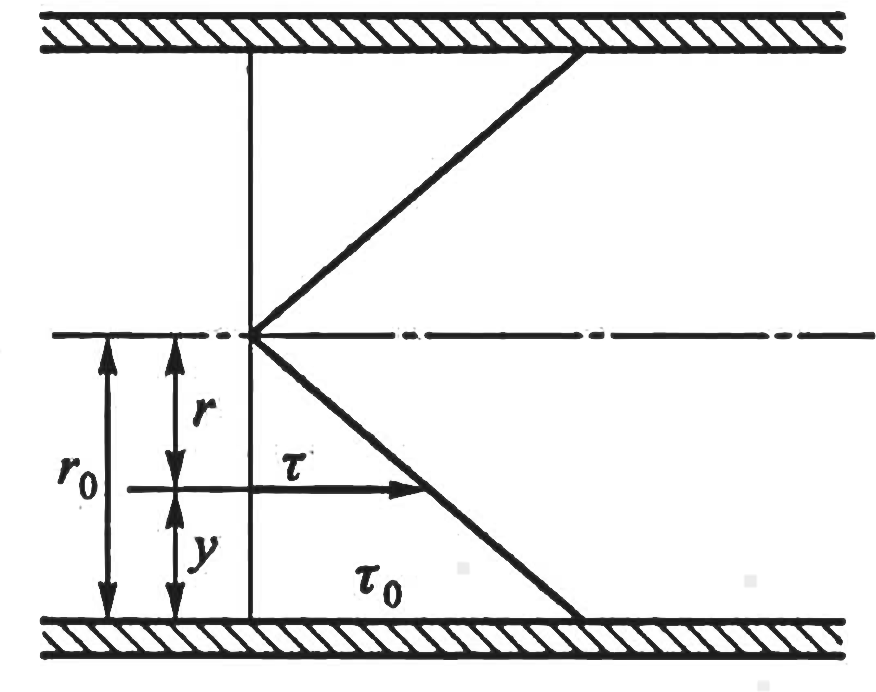
\includegraphics[width=\linewidth,height=0.46\textheight,keepaspectratio]{slides_assets/fluid_deck06/circ-shear.png}\\
      {\scriptsize 图：源讲义原图}
  \end{columns}
  层流时 $\tau$ 是粘性切应力；紊流时 $\tau=\tau_{\text{粘性}}+\tau_{\text{Reynolds}}$，两者之和仍满足线性分布。
  \TLtakeaway{圆管总切应力在中心为零、在壁面最大；该线性分布对均匀层流和均匀紊流都成立。}
\end{frame}

\begin{frame}{C7 宽矩形明渠：从床面到水面线性减小}
  进度：继续使用 $\tau=\rho gR'J$；本帧把内部子区域换成宽矩形明渠中的上部水层。\proofskipnote
  \begin{columns}[T]
    \column{0.52\textwidth}
      设明渠宽度 $B\gg H$，水深为 $H$。令 $y$ 自床面向自由水面量起，则位于高度 $y$ 以上的流体厚度为 $H-y$：
      \[
        A'=B(H-y),\qquad \chi'\approx B,\qquad R'\approx H-y.
      \]
      于是
      \[
        \tau=\rho g(H-y)J
        =\tau_w\left(1-\frac{y}{H}\right),
        \qquad \tau_w=\rho gHJ.
        \tag{H5}
      \]
    \column{0.48\textwidth}
      \centering
      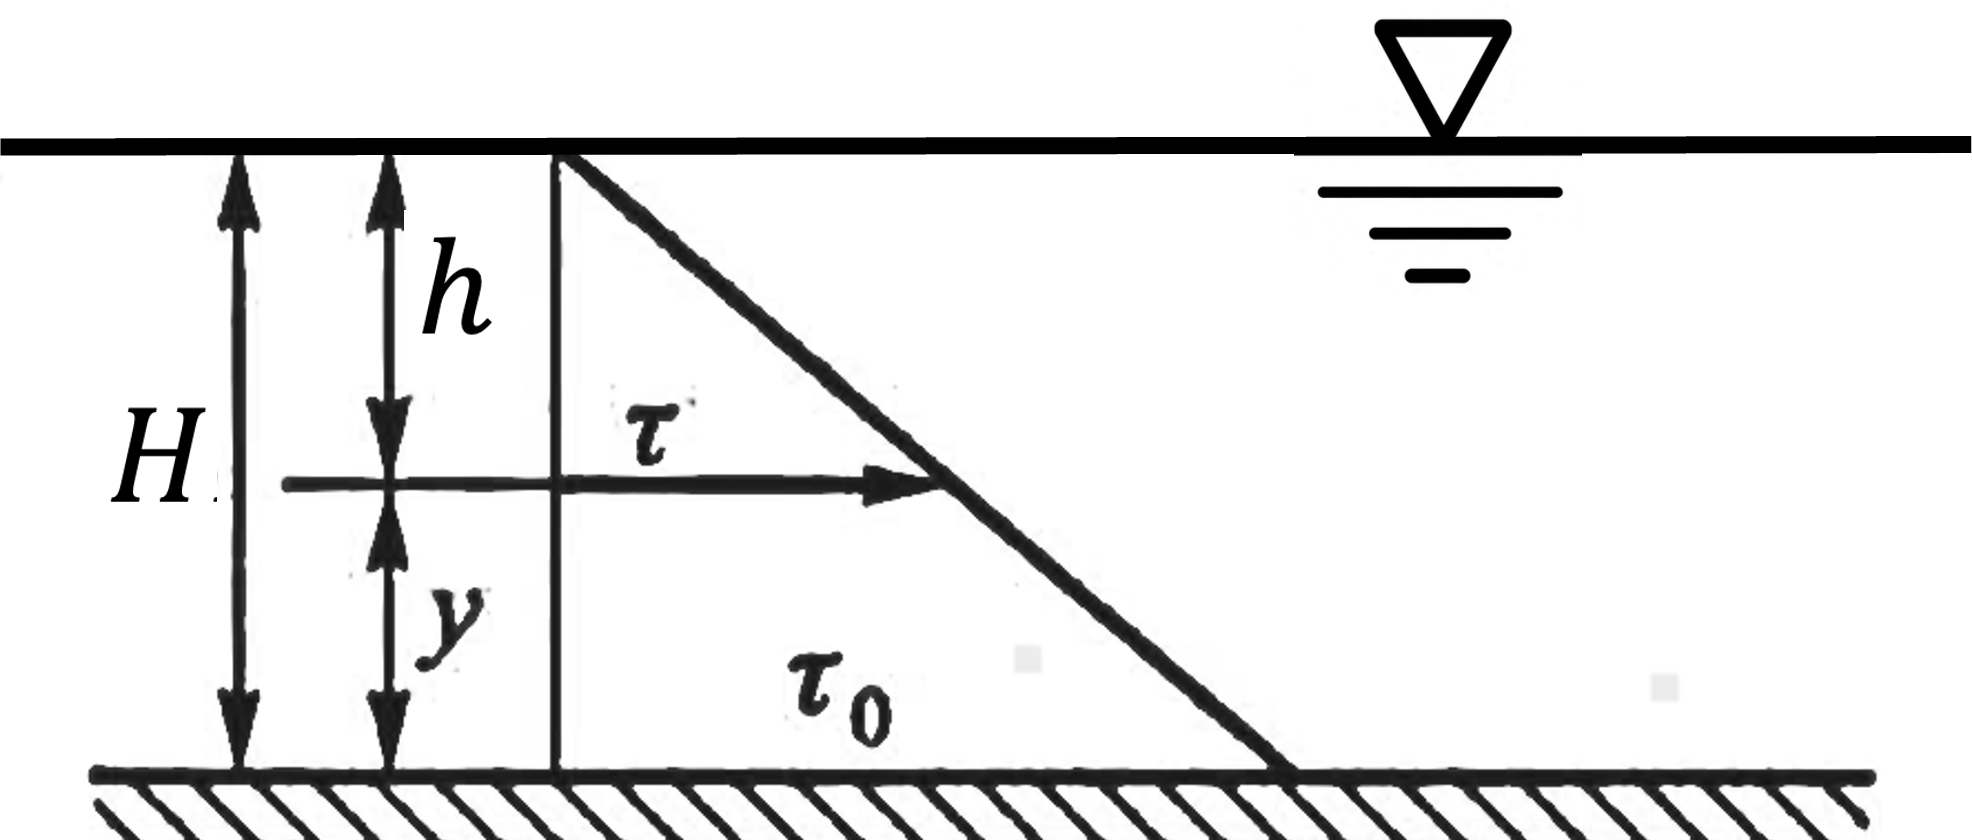
\includegraphics[width=\linewidth,height=0.62\textheight,keepaspectratio]{slides_assets/fluid_deck06/channel-shear.png}\\
      {\scriptsize 图：源讲义原图}
  \end{columns}
  \TLtakeaway{宽矩形明渠的总切应力在床面最大、在自由水面为零；公式中的 $y$ 必须按图从床面量起。}
\end{frame}

\begin{frame}{C8 圆管层流速度分布：联立牛顿内摩擦律}
  进度：圆管切应力已经由 (H4) 给出；本帧只把层流的牛顿内摩擦律与 (H4) 联立成微分方程。\proofskipnote
  \begin{columns}[T]
    \column{0.52\textwidth}
      层流中切应力由分子粘性给出。半径坐标 $r$ 从管心指向壁面，而 Deck 1 的 $y$ 从壁面指向管心，所以 $\rd y=-\rd r$：
      \[
        \tau=\mu\dd{u}{y}
        =-\mu\dd{u}{r}.
      \]
      与 (H4) 的 $\tau=\frac12\rho grJ$ 相等，得到
      \[
        -\mu\dd{u}{r}=\frac12\rho grJ,
        \qquad
        \dd{u}{r}=-\frac{\rho gJ}{2\mu}r.
      \]
    \column{0.48\textwidth}
      \centering
      \begin{tikzpicture}[scale=0.78,>={Stealth[length=5pt]}]
        \draw[fill=TLprimaryTint,draw=TLprimary,thick] (0,0) circle (1.25);
        \draw[->,TLprimaryDark,thick] (0,0)--(1.25,0) node[midway,above] {$r$};
        \draw[->,TLaccent,thick] (1.25,0)--(0.35,0) node[midway,below] {$y$};
        \draw[TLprimaryDark,thick] (-1.25,-1.45)--(1.25,-1.45) node[right] {壁面};
        \draw[TLaccent,thick,smooth,domain=-1:1,samples=80]
          plot({1.15*(1-\x*\x)}, {1.1*\x});
        \node[TLinkSoft,align=center,text width=4.8cm] at (0,-2.05)
          {$r$ 增大时更靠近壁面，速度 $u$ 下降，所以 $\mathrm du/\mathrm dr<0$。};
      \end{tikzpicture}
  \end{columns}
  \TLtakeaway{负号来自坐标方向：$r$ 向外、速度向壁面减小；不是人为调符号。}
\end{frame}

\begin{frame}{C9 积分求圆管层流速度剖面}
  进度：上一帧得到 $\mathrm du/\mathrm dr=-(\rho gJ/2\mu)r$；本帧只积分并代入无滑移边界条件。\proofskipnote
  \begingroup
  \setlength{\abovedisplayskip}{2pt}
  \setlength{\belowdisplayskip}{2pt}
  \setlength{\abovedisplayshortskip}{2pt}
  \setlength{\belowdisplayshortskip}{2pt}
  \setlength{\jot}{1pt}
  \[
    \begin{aligned}
    \dd{u}{r}&=-\frac{\rho gJ}{2\mu}r,\\
    u&=-\frac{\rho gJ}{4\mu}r^2+C.
    \end{aligned}
  \]
  壁面无滑移条件是 $u(r_0)=0$，所以
  \[
    0=-\frac{\rho gJ}{4\mu}r_0^2+C
    \quad\Longrightarrow\quad
    C=\frac{\rho gJ}{4\mu}r_0^2.
  \]
  因此
  \[
    u(r)=\frac{\rho gJ}{4\mu}\left(r_0^2-r^2\right),
    \qquad
    u_{\max}=\frac{\rho gJr_0^2}{4\mu}
    =\frac{\rho gJd^2}{16\mu}.
    \tag{H6}
  \]
  \begin{center}
    \vspace{-0.7em}
    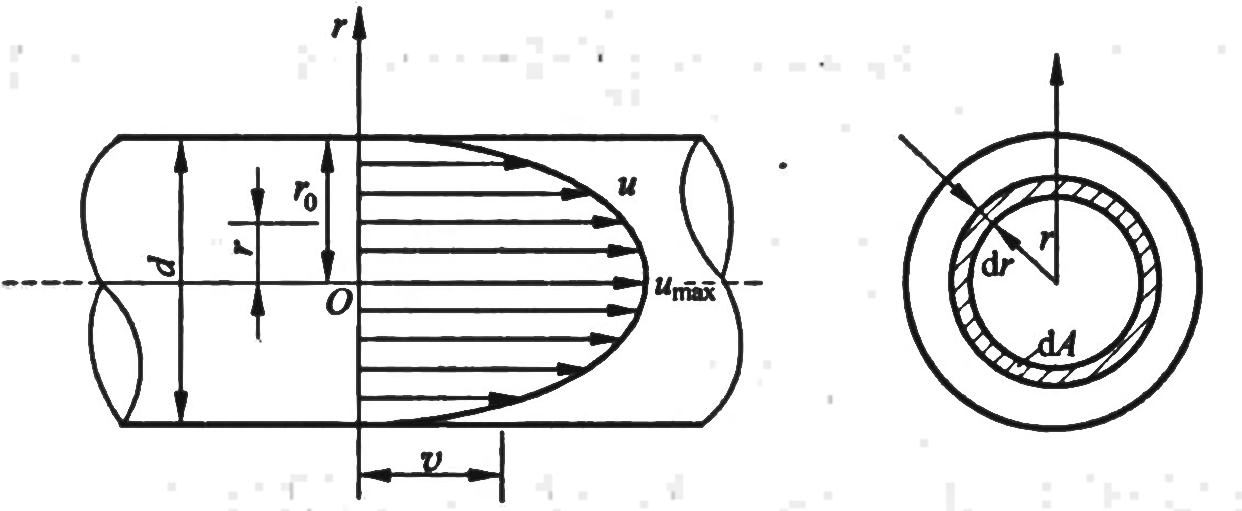
\includegraphics[width=0.72\textwidth,height=0.02\textheight,keepaspectratio]{slides_assets/fluid_deck06/laminar-profile.png}\\
    {\scriptsize 图：源讲义原图}
    \vspace{-0.7em}
  \end{center}
  \endgroup
  \TLtakeaway{圆管层流速度剖面是旋转抛物面；最大速度在管心，壁面速度由无滑移条件固定为零。}
\end{frame}

\begin{frame}{C10 断面平均流速：积分得到 $v=u_{\max}/2$}
  进度：已经有局部速度 $u(r)$；本帧只做面积平均，得到可测的断面平均流速 $v$。\proofskipnote
  \[
    \begin{aligned}
    v
    &=\frac{1}{\pi r_0^2}
      \int_{0}^{r_0}
      \frac{\rho gJ}{4\mu}\left(r_0^2-r^2\right)\,2\pi r\,\rd r\\
    &=\frac{\rho gJ}{2\mu r_0^2}
      \left[\frac{r_0^2r^2}{2}-\frac{r^4}{4}\right]_{0}^{r_0}\\
    &=\frac{\rho gJr_0^2}{8\mu}
     =\frac{\rho gJd^2}{32\mu}
     =\frac{u_{\max}}{2}.
    \end{aligned}
    \tag{H7}
  \]
  \TLtakeaway{平均速度比最大速度小一半；后面求水头损失时用 $v$，因为它可由流量 $Q=vA$ 直接测得。}
\end{frame}

\begin{frame}{C11 圆管层流水头损失：由 $v$ 反求 $J$}
  进度：上一帧得到 $v=\rho gJd^2/(32\mu)$；本帧只把它反解为水力坡度，再乘以管长。\proofskipnote
  \[
    v=\frac{\rho gJd^2}{32\mu}
    \quad\Longrightarrow\quad
    J=\frac{32\mu v}{\rho gd^2}.
  \]
  因为 $J=h_f/l$，所以长为 $l$ 的圆管层流沿程水头损失为
  \[
    h_f=Jl
    =\frac{32\mu vl}{\rho gd^2}.
    \tag{H8}
  \]
  \begin{columns}[T]
    \column{0.50\textwidth}
      \begin{itemize}
        \item $\mu$ 越大，粘性耗散越强，$h_f$ 越大。
        \item $l$ 越长，摩擦作用距离越长，$h_f$ 越大。
      \end{itemize}
    \column{0.50\textwidth}
      \begin{itemize}
        \item $d$ 出现在平方分母中，小管径会显著增加损失。
        \item 层流中 $h_f$ 与 $v$ 成一次方正比。
      \end{itemize}
  \end{columns}
  \TLtakeaway{Hagen--Poiseuille 的水头形式说明：圆管层流不是 $v^2$ 律，而是 $h_f\propto v$。}
\end{frame}

\begin{frame}{C12 层流沿程损失系数：$\lambda=64/\Rey$}
  进度：已经有层流解析式 (H8)；本帧把它写成达西形式，读出层流的 $\lambda$。\proofskipnote
  达西形式先写为
  \[
    h_f=\lambda\frac{l}{d}\frac{v^2}{2g}.
  \]
  令它与 (H8) 相等：
  \[
    \lambda\frac{l}{d}\frac{v^2}{2g}
    =
    \frac{32\mu vl}{\rho gd^2}.
  \]
  两边同除以 $(l/d)(v^2/2g)$，得到
  \[
    \lambda
    =\frac{64\mu}{\rho vd}
    =\frac{64}{\rho vd/\mu}
    =\frac{64}{\Rey}.
    \tag{H9}
  \]
  \TLtakeaway{层流中 $\lambda=64/\Rey$，完全由 $\Rey$ 决定，与壁面粗糙度无关。}
\end{frame}

\begin{frame}{C13a 达西--威斯巴赫公式：圆管通用形式}
  进度：层流给出了 $\lambda=64/\Rey$；工程上把同一形式推广到充分发展圆管流，用不同的 $\lambda$ 表示不同阻力状态。
  \textbf{半经验公式（紊流 $\lambda$ 拟合对象：实验数据；适用假设：完全发展流）。}
  \[
    h_f=\lambda\frac{l}{d}\frac{v^2}{2g}.
    \tag{H10}
  \]
  \begin{center}
  \begin{tikzpicture}[scale=0.74,>={Stealth[length=5pt]}]
    \draw[fill=TLprimaryTint,draw=TLprimary,thick,rounded corners=5pt] (-3.3,-0.45) rectangle (3.3,0.45);
    \draw[->,TLprimaryDark,thick] (-2.9,0)--(-1.6,0) node[above] {$v$};
    \draw[<->,TLinkSoft,thick] (-3.3,-0.78)--(3.3,-0.78) node[midway,below] {$l$};
    \draw[<->,TLinkSoft,thick] (3.65,-0.45)--(3.65,0.45) node[midway,right] {$d$};
    \node[draw=TLaccent,fill=TLaccentLight,rounded corners=2pt,align=center] at (0,1.35)
      {$\lambda$ 把壁面状态、流态和经验数据压缩成一个无量纲系数};
  \end{tikzpicture}
  \end{center}
  \TLtakeaway{达西公式的形式统一；真正需要判断的是 $\lambda$ 处在哪个流动区。}
\end{frame}

\begin{frame}{C13b 任意断面：用 $4R$ 替代圆管直径}
  圆管的水力半径是 $R=d/4$，所以 $d=4R$。对任意过水断面，工程上用 $4R$ 作等效水力直径。
  \[
    h_f=\lambda\frac{l}{4R}\frac{v^2}{2g}.
    \tag{H11}
  \]
  对层流圆管，$\lambda=64/\Rey$ 来自解析推导；对紊流，$\lambda$ 不能只靠牛顿内摩擦律解出，通常写成
  \[
    \lambda=f\!\left(\Rey,\frac{\Delta}{d}\right),
    \qquad
    \text{由实验公式或穆迪图确定。}
    \tag{H12}
  \]
  \begin{center}
  \begin{tikzpicture}[scale=0.68,>={Stealth[length=5pt]}]
    \draw[fill=TLprimaryTint,draw=TLprimary,thick] (-3.0,0) circle (0.82);
    \node at (-3.0,-1.2) {圆管：$d=4R$};
    \draw[fill=TLprimaryTint,draw=TLprimary,thick,rounded corners=2pt] (-0.8,-0.55) rectangle (1.0,0.65);
    \node at (0.1,-1.2) {箱涵：算 $R=A/\chi$};
    \draw[fill=TLprimaryTint,draw=TLprimary,thick] (2.4,-0.4) .. controls (3.0,0.9) and (4.0,0.65) .. (4.25,-0.35) -- cycle;
    \node at (3.35,-1.2) {明渠：湿周不含自由面};
  \end{tikzpicture}
  \end{center}
  \TLtakeaway{非圆断面不是重新发明公式，而是先算 $R=A/\chi$，再用 $4R$ 替代圆管直径。}
\end{frame}

\begin{frame}{C13c 速度幂律：什么时候才有 $h_f\propto v^2$}
  达西公式含有 $v^2$，但 $\lambda$ 本身可能随 $v$ 变；所以不能直接说所有沿程损失都与速度平方成正比。
  \[
    h_f=kv^n,\qquad
    \begin{cases}
      n=1, & \text{圆管层流，因为 }\lambda=64/\Rey\propto v^{-1},\\
      n\approx1.75\text{--}2, & \text{紊流中 }\lambda\text{ 变化较慢},\\
      n=2, & \text{阻力平方区，}\lambda\approx\text{常数}.
    \end{cases}
    \tag{H13}
  \]
  \TLwarnblock{常见误区}{
    看到达西公式里的 $v^2$ 就断言 $h_f\propto v^2$，会把层流和光滑紊流都判断错。必须先问 $\lambda$ 是否可近似看成常数。
  }
  \TLtakeaway{$h_f\propto v^2$ 仅在 $\lambda\approx\mathrm{const}$（粗糙紊流阻力平方区）时成立；层流 $h_f\propto v^1$。}
\end{frame}

% =============================================================================
% D. 5.4 沿程损失系数的变化规律
% =============================================================================
\TLsection{5.4 沿程损失系数的变化规律}

\begin{frame}{D1 $u_*$ 与 $\lambda$ 的关系}
  目的：Deck 5 用\TLterm{摩阻流速} $u_*$ 描述近壁尺度；本帧把它改写成可查表得到的 $\lambda$。
  \begin{columns}[T]
    \column{0.58\textwidth}
      \small
      \[
        u_*=\sqrt{\frac{\tau_w}{\rho}}
        =\sqrt{gRJ}
        \tag{H14}
      \]
      由达西--威斯巴赫公式反解 $J$：
      \[
        J=\frac{h_f}{l}
        =\lambda\frac{1}{4R}\frac{v^2}{2g}.
      \]
      代入 (H14)：
      \[
        u_*^2=gR\cdot\lambda\frac{1}{4R}\frac{v^2}{2g}
        =\frac{\lambda v^2}{8},
        \qquad
        u_*=v\sqrt{\frac{\lambda}{8}}.
        \tag{H15}
      \]
      \[
        \delta'=14.1\frac{d}{\Rey\sqrt{\lambda}},\qquad
        \delta=32.8\frac{d}{\Rey\sqrt{\lambda}}.
        \tag{H16}
      \]
    \column{0.42\textwidth}
      \centering
      \begin{tikzpicture}[scale=0.62,>={Stealth[length=5pt]}]
        \draw[fill=TLprimaryTint,draw=TLprimary,thick] (0,0) circle (1.38);
        \draw[fill=white,draw=TLprimaryLight,thick] (0,0) circle (1.00);
        \draw[fill=white,draw=TLaccent,thick,dashed] (0,0) circle (1.20);
        \node[TLprimaryDark] at (0,0) {核心紊流};
        \node[TLaccent,font=\scriptsize] at (1.58,0.34) {$\delta$};
        \node[TLaccent,font=\scriptsize] at (1.54,-0.22) {$\delta'$};
        \draw[<->,TLaccent,thick] (1.20,0.86)--(1.38,0.98);
        \draw[<->,TLaccent,thick] (1.00,-0.70)--(1.38,-0.96);
        \draw[->,TLprimaryDark,thick] (-0.85,0)--(0.85,0) node[midway,above] {$v$};
        \node[TLinkSoft,align=center,text width=3.8cm] at (0,-2.00)
          {$\Rey$ 越大，底层越薄。};
      \end{tikzpicture}
  \end{columns}
  \vspace{-3pt}
  \TLtakeaway{$u_*=v\sqrt{\lambda/8}$ 是由 $\tau_w=\rho gRJ$ 与达西公式推出的关系。}
\end{frame}

\begin{frame}{D2 尼古拉兹实验：把 $\lambda$ 的变化分成五区}
  动机：紊流中 $\lambda$ 不能像层流那样由解析速度剖面给出；尼古拉兹用\TLterm{人工沙粒粗糙管}测得 $\lambda=f(\Rey,\Delta/d)$。
  \begin{columns}[T]
    \column{0.38\textwidth}
      \begin{itemize}
        \item 横轴：$\lg(\Rey)$。
        \item 纵轴：$\lg(100\lambda)$。
        \item 多条曲线：不同相对粗糙度 $\Delta/d$。
        \item 关键问题：每一区域中 $\lambda$ 主要依赖谁。
      \end{itemize}
    \column{0.62\textwidth}
      \centering
      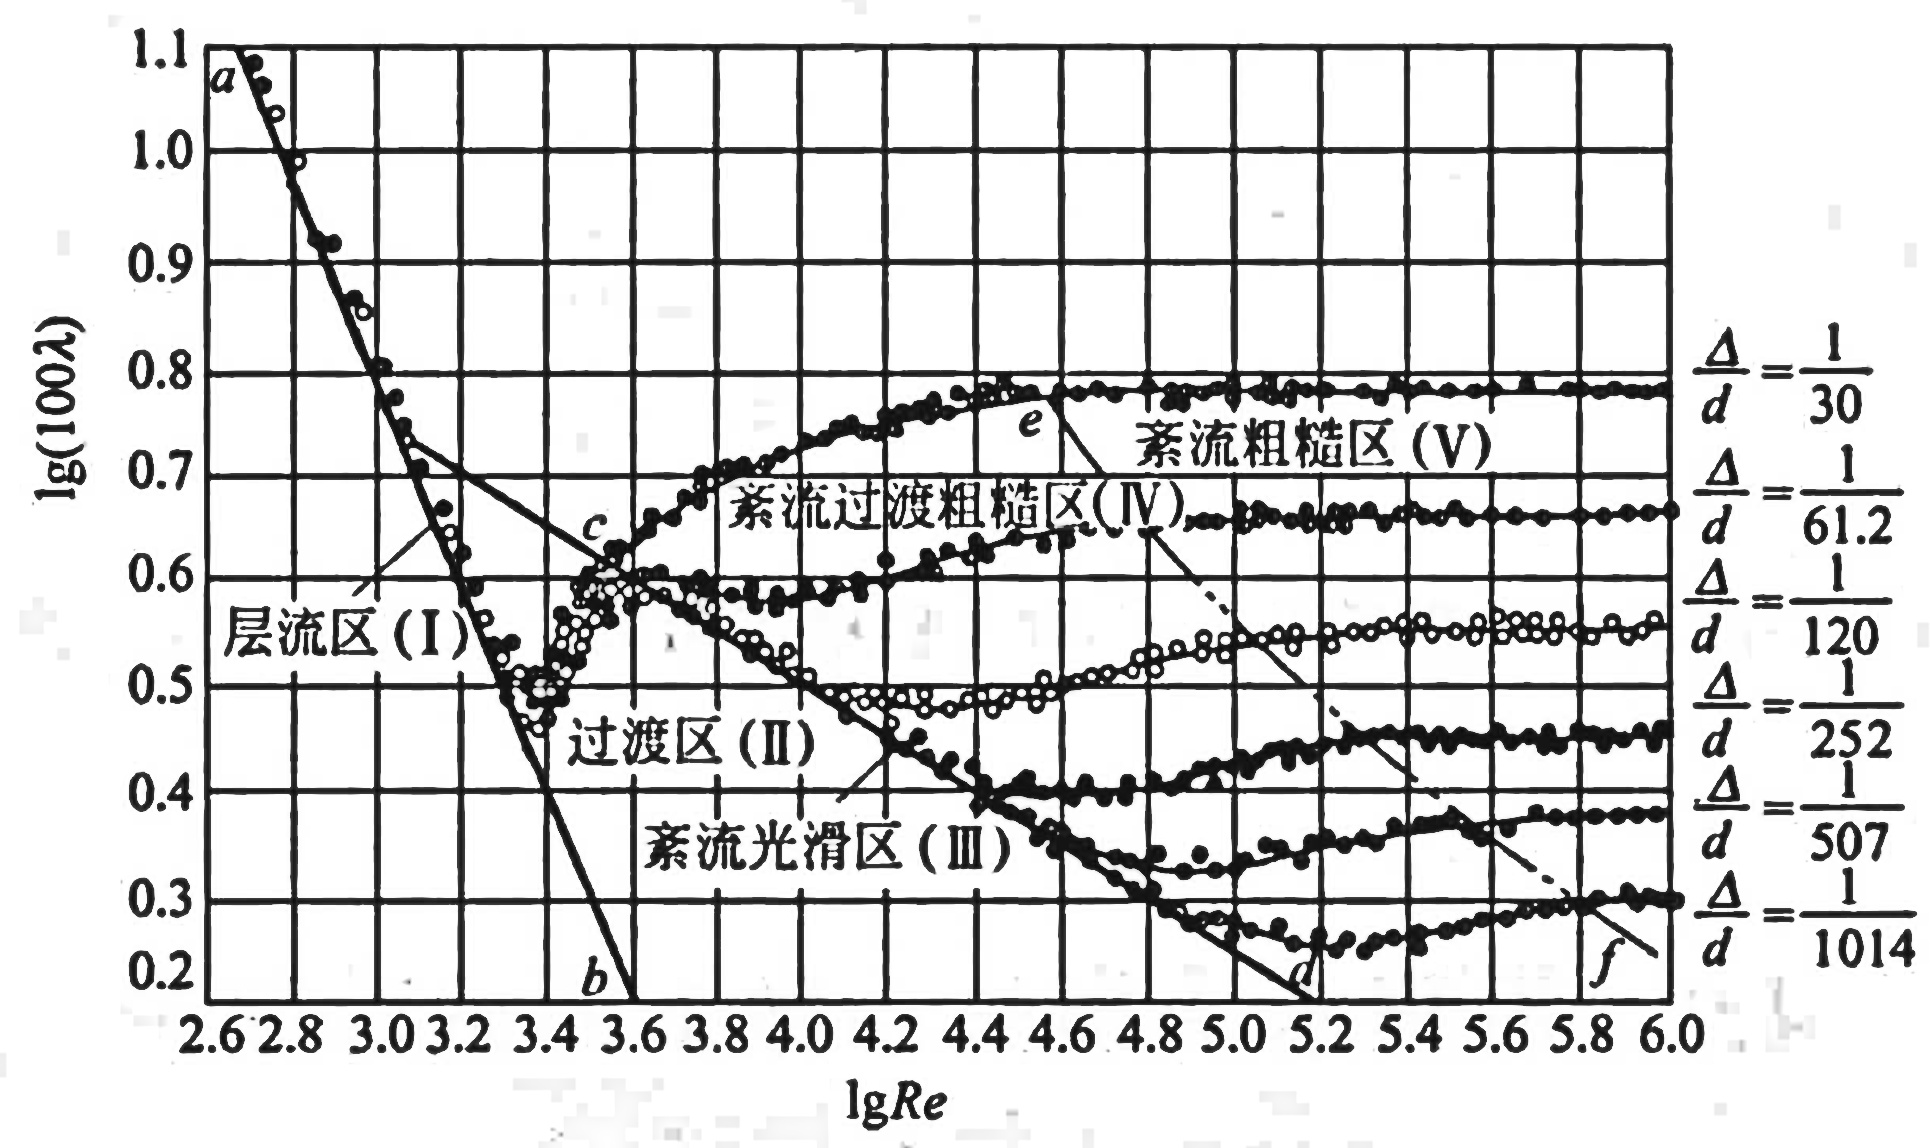
\includegraphics[width=\linewidth,height=0.52\textheight,keepaspectratio]{slides_assets/fluid_deck06/nikuradse.png}\\
      {\scriptsize 图：源讲义原图}
  \end{columns}
  \TLtakeaway{五区的本质是判断 $\lambda$ 依赖 $\Rey$、$\Delta/d$，还是两者都依赖。}
\end{frame}

\begin{frame}{D3 五区公式 I：层流区}
  在 $\Rey<2000$ 时，流动保持层流；圆管速度剖面是抛物面，5.3 已经由解析积分推出沿程损失系数。
  \begin{columns}[T]
    \column{0.54\textwidth}
      \textbf{精确公式（适用：圆管层流区）。}
      \[
        \lambda=\frac{64}{\Rey},
        \qquad \Rey<2000.
        \tag{H17}
      \]
      \begin{itemize}
        \item 只依赖 $\Rey$，与相对粗糙度 $\Delta/d$ 无关。
        \item 因为 $\Rey=\rho vd/\mu$，同一管道中 $\lambda\propto v^{-1}$。
        \item 代回达西公式后，$h_f\propto v$。
      \end{itemize}
    \column{0.46\textwidth}
      \centering
      \begin{tikzpicture}[scale=0.66,>={Stealth[length=5pt]}]
        \draw[fill=TLprimaryTint,draw=TLprimary,thick,rounded corners=5pt] (-2.1,-0.65) rectangle (2.1,0.65);
        \foreach \y in {-0.42,-0.21,0,0.21,0.42}{
          \pgfmathsetmacro{\len}{1.45*(1-(\y/0.62)^2)+0.25}
          \draw[->,TLprimaryDark,thick] (-1.65,\y)--(-1.65+\len,\y);
        }
        \node[TLinkSoft,align=center,text width=4.8cm] at (0,-1.45)
          {层流的剖面可解析积分，所以 $\lambda=64/\Rey$ 是精确结果。};
        \begin{scope}[shift={(0,1.55)}]
          \draw[->,TLprimaryDark,thick] (-1.6,0)--(1.75,0) node[right] {$v$};
          \draw[->,TLprimaryDark,thick] (-1.6,0)--(-1.6,1.15) node[above] {$h_f$};
          \draw[TLaccent,thick] (-1.35,0.12)--(1.35,0.95);
          \node[TLaccent,font=\small] at (0.65,1.08) {$h_f\propto v$};
        \end{scope}
      \end{tikzpicture}
  \end{columns}
  \TLtakeaway{层流中 $\lambda$ 随 $\Rey$ 减小，但总损失仍按 $h_f\propto v$ 增大。}
\end{frame}

\begin{frame}{D4 五区公式 II：层流向紊流过渡区}
  当 $2000<\Rey<4000$ 时，流动可能在层流和紊流之间摆动；扰动、入口条件和管壁状态都会放大成不同结果。
  \begin{columns}[T]
    \column{0.55\textwidth}
      \[
        2000<\Rey<4000:
        \qquad \text{目前没有可靠通用公式。}
        \tag{H18}
      \]
      \begin{itemize}
        \item 实验点分散，$\lambda$ 对 $\Rey$ 的响应不稳定。
        \item 不能把层流公式或紊流公式硬接起来使用。
        \item 工程设计通常把这个区看成需要避开的不稳定区。
      \end{itemize}
    \column{0.45\textwidth}
      \centering
      \begin{tikzpicture}[scale=0.68,>={Stealth[length=5pt]}]
        \draw[->,TLprimaryDark,thick] (-2.0,0)--(2.2,0) node[right] {$\Rey$};
        \draw[->,TLprimaryDark,thick] (-2.0,0)--(-2.0,2.6) node[above] {$\lambda$};
        \draw[TLprimary,thick] (-1.75,2.2)--(-0.65,1.25);
        \foreach \x/\y in {-0.42/1.55,-0.18/1.88,0.10/1.28,0.36/1.75,0.62/1.42,0.92/2.00}{
          \fill[TLaccent] (\x,\y) circle (1.6pt);
        }
        \draw[TLprimary,thick] (1.10,1.65)..controls (1.45,1.35)..(1.85,1.15);
        \draw[dashed,TLinkSoft] (-0.55,0)--(-0.55,2.35);
        \draw[dashed,TLinkSoft] (1.05,0)--(1.05,2.35);
        \node[font=\small,TLinkSoft] at (0.25,-0.35) {$2000$--$4000$};
        \node[align=center,TLinkSoft,text width=3.8cm] at (0,-1.18)
          {数据“散”，说明状态对扰动敏感。};
      \end{tikzpicture}
  \end{columns}
  \TLwarnblock{工程提醒}{本区没有稳定可靠的 $\lambda$ 公式；工程中应避免在此区运行。}
\end{frame}

\begin{frame}{D5 五区公式 III：紊流光滑管区}
  \small
  在\TLterm{水力光滑管}中，壁面粗糙凸起仍被粘性底层淹没，粗糙度 $\Delta/d$ 对 $\lambda$ 的影响可以忽略。
  \begin{columns}[T]
    \column{0.56\textwidth}
      \textbf{半经验公式（适用：紊流光滑管，$\Delta/d$ 对 $\lambda$ 无影响）。}
      \[
        \lambda=\frac{0.3164}{\Rey^{1/4}},
        \qquad 4000<\Rey<10^5.
        \tag{H19}
      \]
      代入达西公式：
      \[
        h_f\propto \lambda v^2\propto v^{-1/4}v^2
        =v^{1.75}.
      \]
      更宽范围可用尼古拉兹光滑管公式：
      \[
        \frac{1}{\sqrt{\lambda}}
        =2\lg(\Rey\sqrt{\lambda})-0.8.
        \tag{H20}
      \]
    \column{0.44\textwidth}
      \centering
      \begin{tikzpicture}[scale=0.62,>={Stealth[length=5pt]}]
        \draw[TLprimaryDark,thick] (-2.3,0)--(2.3,0);
        \foreach \x in {-1.8,-1.1,-0.35,0.45,1.15,1.85}{
          \draw[fill=TLaccent,draw=TLaccent] (\x,0) -- ++(0.18,0.30) -- ++(0.18,-0.30) -- cycle;
        }
        \draw[fill=TLprimaryTint,draw=none,opacity=0.75] (-2.3,0) rectangle (2.3,0.68);
        \draw[TLprimary,thick,dashed] (-2.3,0.68)--(2.3,0.68);
        \node[TLprimaryDark,font=\small] at (0,0.95) {粘性底层 $\delta'>\Delta$};
        \draw[->,TLprimaryDark,thick] (-1.9,1.55)--(-0.6,1.55) node[above] {$v$};
        \node[TLinkSoft,align=center,text width=4.0cm] at (0,-1.05)
          {粗糙凸起被底层遮住，主导因素退化为 $\Rey$。};
      \end{tikzpicture}
  \end{columns}
  \vspace{-3pt}
  \TLtakeaway{光滑紊流中 $\lambda$ 随 $\Rey$ 变，典型幂次是 $h_f\propto v^{1.75}$。}
\end{frame}

\begin{frame}{D6 五区公式 IV：紊流过渡粗糙区}
  \small
  当 $\Rey$ 继续增大时，粘性底层变薄，粗糙凸起开始伸出底层；此时 $\lambda$ 同时受 $\Rey$ 和 $\Delta/d$ 控制。
  \begin{columns}[T]
    \column{0.58\textwidth}
      \textbf{半经验公式（适用：过渡粗糙区）。}
      \[
        \frac{1}{\sqrt{\lambda}}
        =
        -2\lg\!\left(
          \frac{\Delta}{3.71d}
          +
          \frac{2.51}{\Rey\sqrt{\lambda}}
        \right).
        \tag{H21}
      \]
      \begin{itemize}
        \item 第一项来自相对粗糙度 $\Delta/d$。
        \item 第二项来自粘性影响和 $\Rey$。
        \item $\lambda$ 同时出现在两边，必须迭代求解。
      \end{itemize}
    \column{0.42\textwidth}
      \centering
      \begin{tikzpicture}[scale=0.62,>={Stealth[length=5pt]}]
        \draw[TLprimaryDark,thick] (-2.25,0)--(2.25,0);
        \foreach \x/\h in {-1.8/0.40,-1.15/0.55,-0.45/0.36,0.25/0.62,0.95/0.44,1.65/0.58}{
          \draw[fill=TLaccent,draw=TLaccent] (\x,0)--++(0.18,\h)--++(0.18,-\h)--cycle;
        }
        \draw[fill=TLprimaryTint,draw=none,opacity=0.70] (-2.25,0) rectangle (2.25,0.42);
        \draw[TLprimary,thick,dashed] (-2.25,0.42)--(2.25,0.42);
        \node[TLprimaryDark,font=\small] at (0,0.82) {$\delta'$ 与 $\Delta$ 同量级};
        \draw[->,TLprimaryDark,thick] (-1.8,1.38)--(-0.55,1.38) node[above] {$v$};
        \node[TLinkSoft,align=center,text width=4.0cm] at (0,-1.08)
          {壁面既没有完全光滑，也没有完全粗糙。};
      \end{tikzpicture}
  \end{columns}
  \TLtakeaway{过渡粗糙区中，$\lambda$ 同时受 $\Rey$ 和 $\Delta/d$ 控制。}
\end{frame}

\begin{frame}{D7 五区公式 V：紊流粗糙区（阻力平方区）}
  \small
  在\TLterm{完全粗糙区}中，粘性底层远小于粗糙凸起高度；近壁耗散主要由凸起后的分离和掺混控制。
  \begin{columns}[T]
    \column{0.56\textwidth}
      \textbf{半经验公式（适用：完全粗糙区、阻力平方区）。}
      \[
        \lambda
        =
        \frac{1}{\left(2\lg\frac{3.71d}{\Delta}\right)^2}.
        \tag{H22}
      \]
      \begin{itemize}
        \item 只依赖 $\Delta/d$，不再显著依赖 $\Rey$。
        \item 同一管道中 $\lambda\approx\mathrm{const}$。
        \item 达西公式因此退化为 $h_f\propto v^2$。
      \end{itemize}
    \column{0.44\textwidth}
      \centering
      \begin{tikzpicture}[scale=0.64,>={Stealth[length=5pt]}]
        \draw[TLprimaryDark,thick] (-2.2,0)--(2.2,0);
        \foreach \x/\h in {-1.8/0.58,-1.1/0.78,-0.38/0.66,0.36/0.90,1.05/0.72,1.72/0.82}{
          \draw[fill=TLaccent,draw=TLaccent] (\x,0)--++(0.18,\h)--++(0.18,-\h)--cycle;
        }
        \draw[fill=TLprimaryTint,draw=none,opacity=0.62] (-2.2,0) rectangle (2.2,0.25);
        \draw[TLprimary,thick,dashed] (-2.2,0.25)--(2.2,0.25);
        \node[TLprimaryDark,font=\small] at (0,1.15) {$\delta'\ll\Delta$};
        \begin{scope}[shift={(0,-1.45)}]
          \draw[->,TLprimaryDark,thick] (-1.55,0)--(1.7,0) node[right] {$v$};
          \draw[->,TLprimaryDark,thick] (-1.55,0)--(-1.55,1.05) node[above] {$h_f$};
          \draw[TLaccent,thick,smooth,domain=-1.2:1.25,samples=50]
            plot(\x,{0.18+0.40*(\x+1.2)^2});
          \node[TLaccent,font=\small] at (0.55,0.95) {$v^2$};
        \end{scope}
      \end{tikzpicture}
  \end{columns}
  \TLtakeaway{阻力平方区中 $\lambda\approx\mathrm{const}$，所以 $h_f\propto v^2$。}
\end{frame}

\begin{frame}{D8 穆迪图与实用管道}
  \small
  尼古拉兹实验使用人工沙粒粗糙管；实际工程管道的粗糙度来自铸铁、钢、混凝土等材料和制造状态，需要用\TLterm{穆迪图}。
  \begin{columns}[T]
    \column{0.48\textwidth}
      \begin{itemize}
        \item 穆迪图形状类似尼古拉兹图，但粗糙度 $\Delta$ 来自实用管道数据。
        \item 使用步骤：先算 $\Rey$，再查 $\Delta/d$，最后读出 $\lambda$。
        \item 非圆管把直径替换为水力直径：
      \end{itemize}
      \[
        d_h=4R.
        \tag{H23}
      \]
    \column{0.52\textwidth}
      \centering
      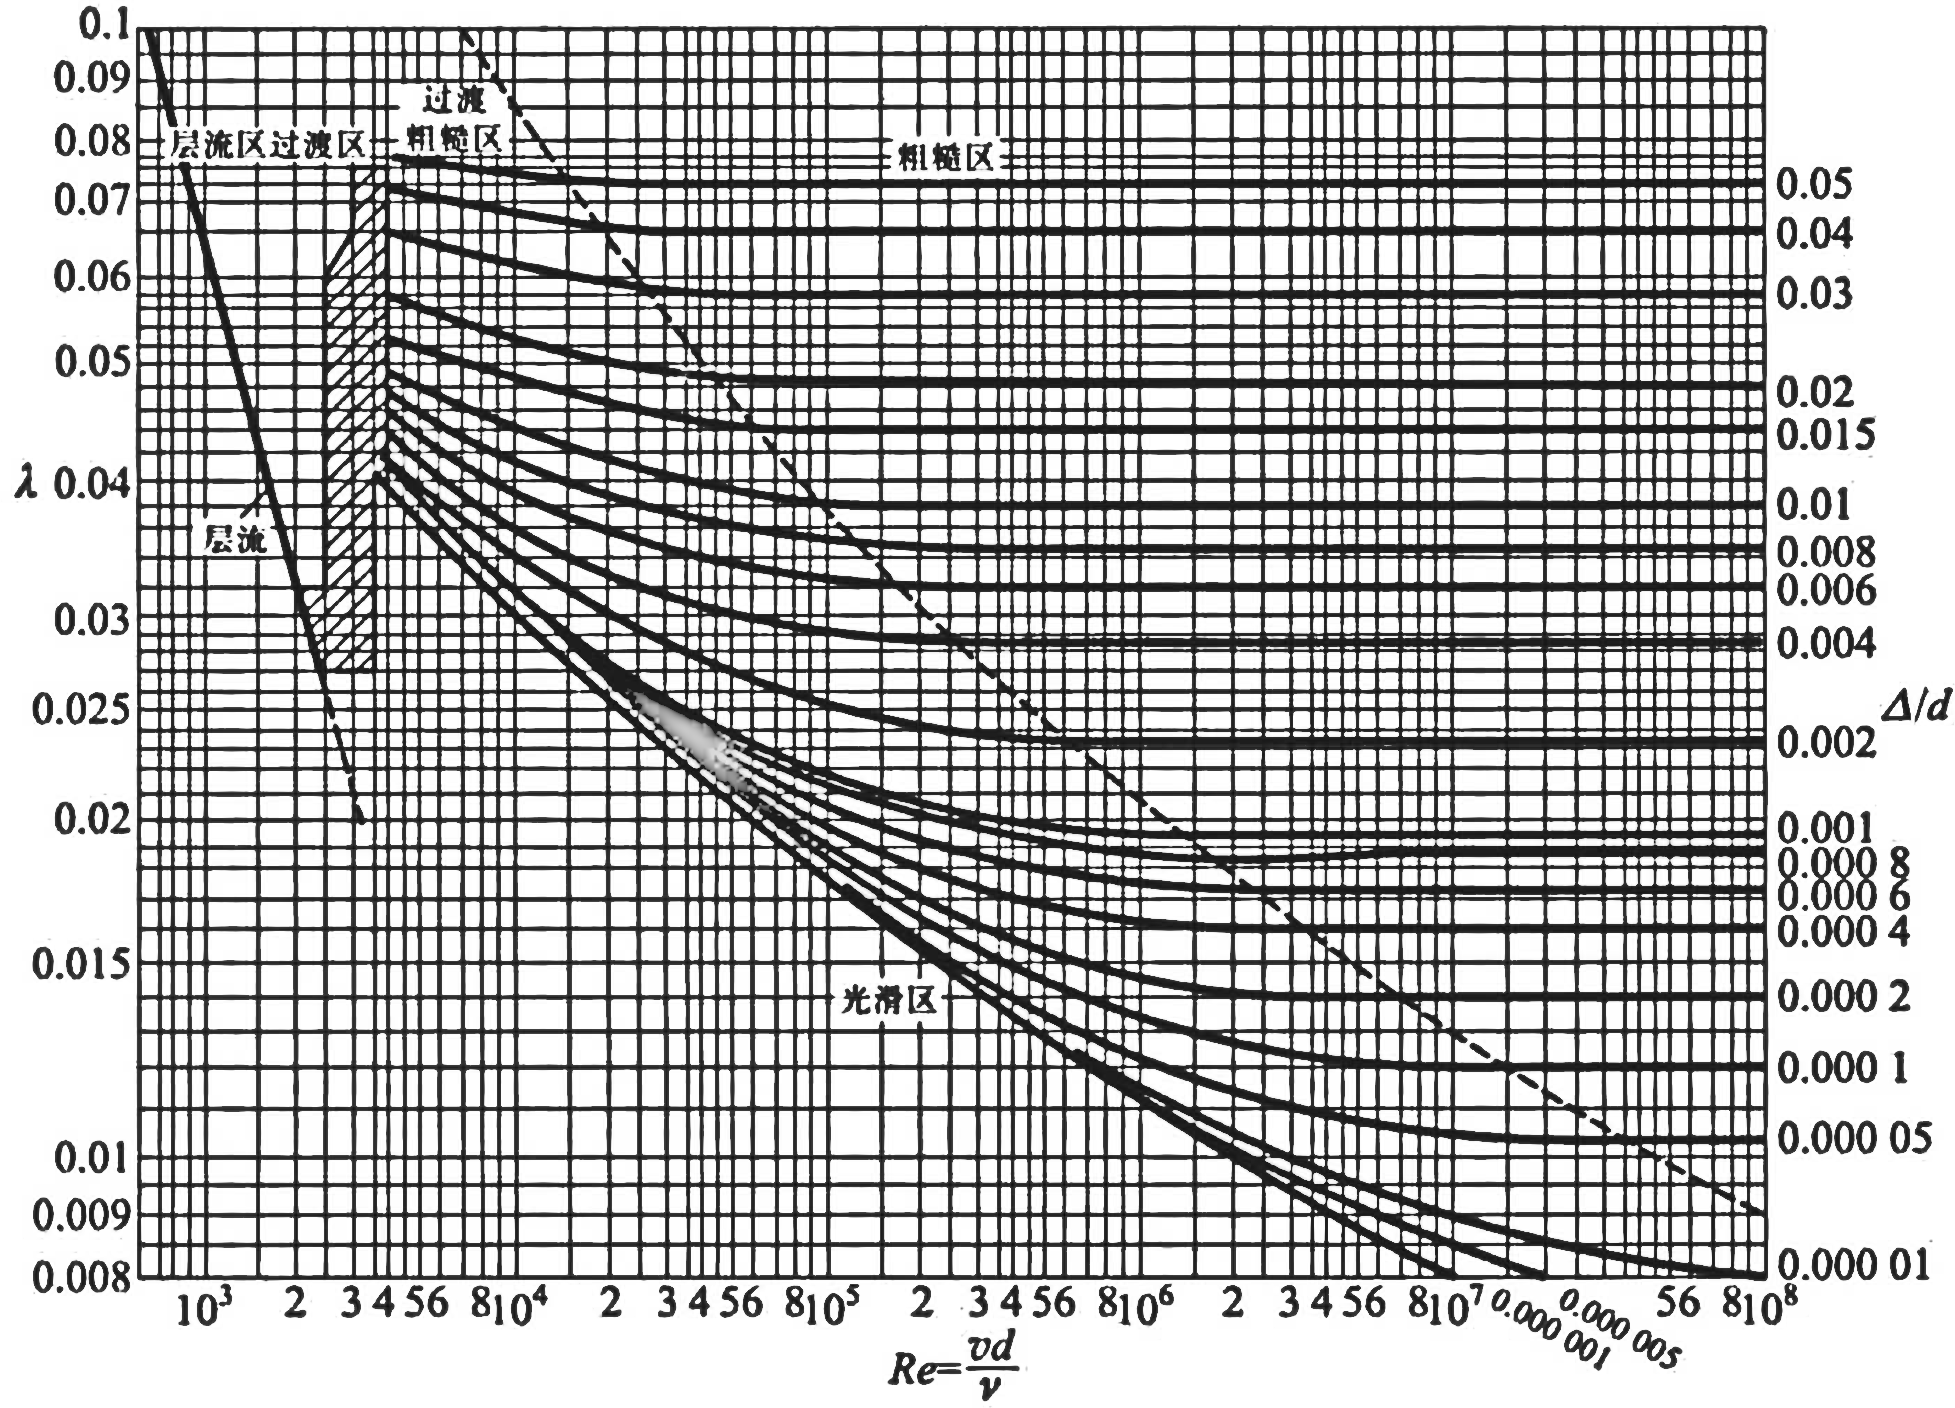
\includegraphics[width=\linewidth,height=0.52\textheight,keepaspectratio]{slides_assets/fluid_deck06/moody.png}\\
      {\scriptsize 图：源讲义原图}
  \end{columns}
  \TLtakeaway{实际工程中优先查穆迪图；非圆断面用 $d_h=4R$。}
\end{frame}

\begin{frame}{D9 谢才公式：与达西公式等价}
  \small
  \TLterm{谢才公式}先在明渠均匀流经验中出现；它把平均流速写成水力半径和水力坡度的函数。
  \begin{columns}[T]
    \column{0.50\textwidth}
      \textbf{经验公式（适用：阻力平方区）。}
      \[
        v=C\sqrt{RJ},
        \qquad
        h_f=Jl=\frac{v^2l}{C^2R}.
        \tag{H24}
      \]
      达西公式在非圆断面写作
      \[
        h_f=\lambda\frac{l}{4R}\frac{v^2}{2g}
        =\frac{\lambda v^2l}{8gR}.
      \]
      对比两式得到
      \[
        C=\sqrt{\frac{8g}{\lambda}},
        \qquad
        \lambda=\frac{8g}{C^2}.
        \tag{H25}
      \]
    \column{0.50\textwidth}
      \centering
      \begin{tikzpicture}[scale=0.66,>={Stealth[length=5pt]}]
        \node[draw=TLprimary,fill=TLprimaryTint,rounded corners=2pt,align=center,text width=4.1cm] (d) at (0,1.55)
          {达西\\$h_f=\lambda l v^2/(8gR)$};
        \node[draw=TLaccent,fill=TLaccentLight,rounded corners=2pt,align=center,text width=4.1cm] (c) at (0,-0.10)
          {谢才\\$h_f=v^2l/(C^2R)$};
        \draw[<->,TLprimaryDark,thick] (d)--(c) node[midway,right] {同一 $h_f$};
        \node[TLinkSoft,align=center,text width=4.6cm] at (0,-1.75)
          {两种写法等价；只是把阻力信息放在 $\lambda$ 或 $C$ 中。};
      \end{tikzpicture}
  \end{columns}
  \TLtakeaway{阻力平方区中，谢才公式与达西公式只是系数互换。}
\end{frame}

\begin{frame}{D10 曼宁公式：给谢才系数一个工程估计}
  \small
  谢才公式还需要 $C$；工程上常用\TLterm{曼宁公式}用水力半径和糙率 $n$ 估计 $C$。
  \begin{columns}[T]
    \column{0.54\textwidth}
      \textbf{经验公式（适用：明渠及阻力平方区管流）。}
      \[
        C=\frac{R^{1/6}}{n},
        \qquad
        n:\ \mathrm{m}^{-1/3}\!\cdot\!\mathrm{s}.
        \tag{H26}
      \]
      与谢才公式合并：
      \[
        v=\frac{1}{n}R^{2/3}J^{1/2}.
        \tag{H27}
      \]
      巴甫洛夫斯基公式也用 $n$ 估计 $C$，常见适用范围为
      $0.1\le R\le3.0\,\mathrm m$。
    \column{0.46\textwidth}
      \centering
      \begin{tikzpicture}[scale=0.64,>={Stealth[length=5pt]}]
        \draw[fill=TLprimaryTint,draw=TLprimary,thick] (-2.1,0) rectangle (2.1,1.35);
        \draw[TLprimaryDark,thick] (-2.35,0)--(2.35,0);
        \draw[TLaccent,thick] (-1.8,0)--(-1.55,0.15)--(-1.30,0)--(-1.05,0.20)--(-0.80,0)
          --(-0.50,0.12)--(-0.25,0)--(0.05,0.18)--(0.35,0)--(0.70,0.14)--(1.0,0)
          --(1.35,0.18)--(1.70,0)--(2.0,0.12);
        \draw[->,TLprimaryDark,thick] (-1.65,0.75)--(-0.45,0.75) node[above] {$v$};
        \draw[<->,TLinkSoft,thick] (2.45,0)--(2.45,1.35) node[midway,right] {$R$};
        \node[TLinkSoft,align=center,text width=4.4cm] at (0,-1.05)
          {$n$ 汇总壁面粗糙、边界形状和其他经验因素。};
      \end{tikzpicture}
  \end{columns}
  \TLwarnblock{量纲提醒}{曼宁公式是量纲不齐次的经验式；使用时 $R$ 必须取米。}
\end{frame}

% =============================================================================
% E. 5.5 局部水头损失
% =============================================================================
\TLsection{5.5 局部水头损失}

\begin{frame}{E1 局部水头损失通用公式}
  \small
  局部构件会让速度方向、断面面积或流线形状突然改变；流动分离和掺混把一部分机械能耗散掉。
  \begin{columns}[T]
    \column{0.52\textwidth}
      \[
        h_j=\zeta\frac{v^2}{2g}.
        \tag{H28}
      \]
      \begin{itemize}
        \item $\zeta$ 是\TLterm{局部损失系数}，无量纲。
        \item $\zeta$ 通常由实验表格或局部理论推导给出。
        \item 若构件前后管径不同，表格必须说明 $v$ 取前断面还是后断面。
      \end{itemize}
    \column{0.48\textwidth}
      \centering
      \begin{tikzpicture}[scale=0.66,>={Stealth[length=5pt]}]
        \draw[TLprimaryDark,thick] (-2.7,0.50)--(-0.25,0.50)--(0.45,0.85)--(2.70,0.85);
        \draw[TLprimaryDark,thick] (-2.7,-0.50)--(-0.25,-0.50)--(0.45,-0.85)--(2.70,-0.85);
        \draw[->,TLprimary,thick] (-2.25,0)--(-1.15,0) node[above] {$v_1$};
        \draw[->,TLprimary,thick] (0.95,0)--(2.05,0) node[above] {$v_2$};
        \draw[TLaccent,thick] (0.28,0.58)..controls (0.65,0.20) and (0.68,-0.20)..(0.28,-0.58);
        \node[TLaccent,font=\small] at (0.85,1.35) {$\zeta_1$ 用 $v_1$?};
        \node[TLaccent,font=\small] at (0.85,-1.35) {$\zeta_2$ 用 $v_2$?};
      \end{tikzpicture}
  \end{columns}
  \TLtakeaway{使用 $\zeta$ 前先核对速度基准。}
\end{frame}

\begin{frame}{E2a 突然扩大：控制体与假设}
  \small
  \TLterm{突然扩大}是少数能给出清晰理论推导的局部损失；关键是把扩大后的回流死水区也纳入受力图像。
  \begin{columns}[T]
    \column{0.54\textwidth}
      三个假设必须同时说明：
      \begin{enumerate}
        \item 忽略扩大区壁面摩擦，不计该短段沿程损失。
        \item 断面 1 位于环形死水区前，$p_1$ 按静压分布并等效作用在全断面 $A_2$ 上。
        \item 动能和动量修正系数均取 $1$，即 $\alpha_1=\alpha_2=1$。
      \end{enumerate}
      连续方程先给出速度关系：
      \[
        A_1v_1=A_2v_2=Q.
        \tag{H29}
      \]
    \column{0.46\textwidth}
      \centering
      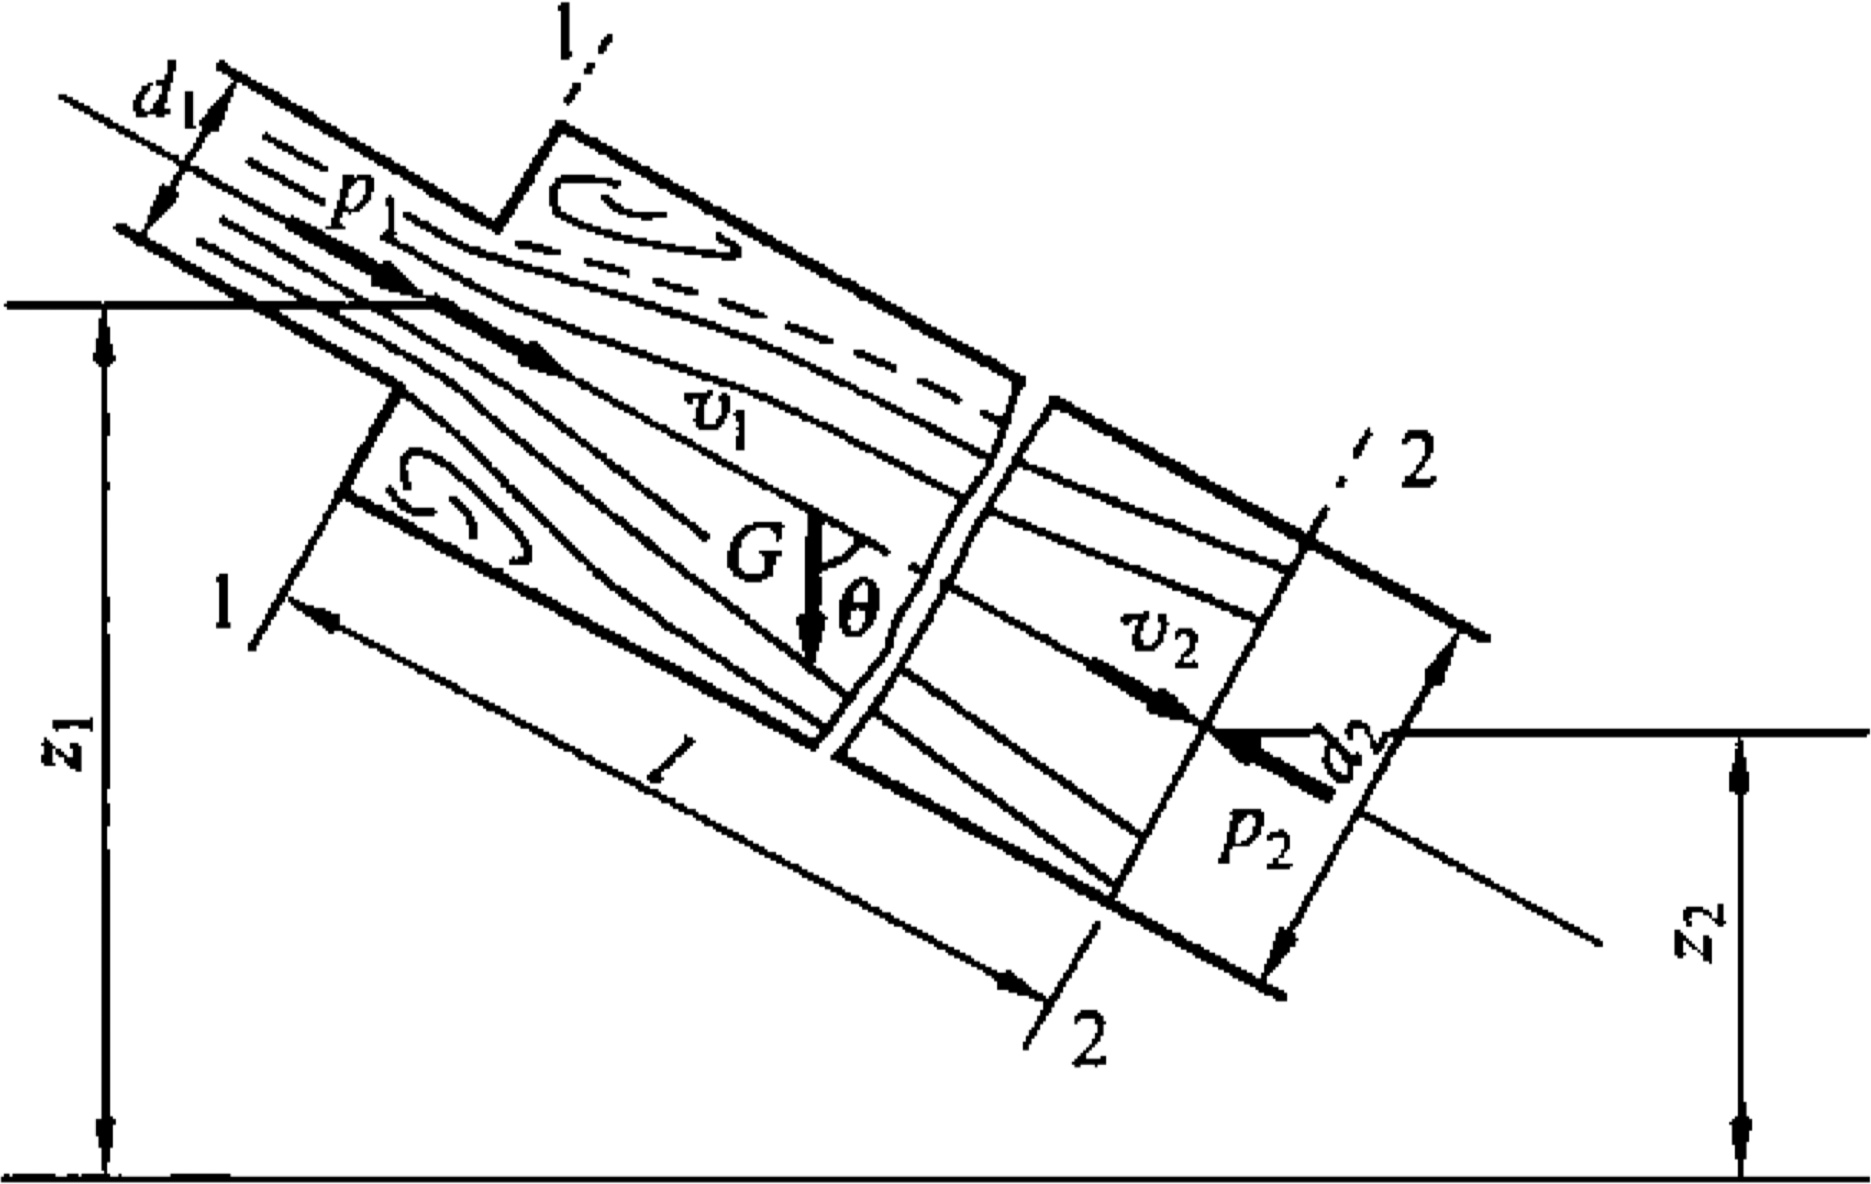
\includegraphics[width=\linewidth,height=0.62\textheight,keepaspectratio]{slides_assets/fluid_deck06/sudden-expansion.png}\\
      {\scriptsize 图：源讲义原图}
  \end{columns}
  \TLtakeaway{突扩推导使用连续、动量、能量三条方程。}
\end{frame}

\begin{frame}{E2b 突然扩大：由动量与能量方程求 $h_j$}
  \small
  进度：上一帧给出 $A_1v_1=A_2v_2=Q$；本帧把压强差从动量方程代入能量方程。
  \[
    p_1A_2-p_2A_2=\rho Q(v_2-v_1).
    \tag{H30}
  \]
  因为 $Q=A_2v_2$，两边除以 $\rho gA_2$：
  \[
    \frac{p_1-p_2}{\rho g}
    =
    \frac{v_2(v_2-v_1)}{g}.
    \tag{H31}
  \]
  两断面能量方程为
  \[
    \frac{p_1}{\rho g}+\frac{v_1^2}{2g}
    =
    \frac{p_2}{\rho g}+\frac{v_2^2}{2g}+h_j.
    \tag{H32}
  \]
  所以
  \[
    h_j=\frac{p_1-p_2}{\rho g}+\frac{v_1^2-v_2^2}{2g}
    =\frac{(v_1-v_2)^2}{2g}.
    \tag{H33}
  \]
  \TLtakeaway{消去压强差即可得到突扩损失。}
\end{frame}

\begin{frame}{E2c 突然扩大：两个速度基准的 $\zeta$}
  \small
  进度：上一帧得到 $h_j=(v_1-v_2)^2/(2g)$；本帧只把同一个损失改写成不同速度基准下的 $\zeta$。
  \begin{columns}[T]
    \column{0.50\textwidth}
      用扩大前速度 $v_1$ 作基准。由 (H29) 有 $v_2=(A_1/A_2)v_1$：
      \[
        h_j
        =
        \left(1-\frac{A_1}{A_2}\right)^2
        \frac{v_1^2}{2g},
        \qquad
        \zeta_1=\left(1-\frac{A_1}{A_2}\right)^2.
        \tag{H34}
      \]
    \column{0.50\textwidth}
      用扩大后速度 $v_2$ 作基准。由 (H29) 有 $v_1=(A_2/A_1)v_2$：
      \[
        h_j
        =
        \left(\frac{A_2}{A_1}-1\right)^2
        \frac{v_2^2}{2g},
        \qquad
        \zeta_2=\left(\frac{A_2}{A_1}-1\right)^2.
        \tag{H35}
      \]
  \end{columns}
  \begin{center}
  \begin{tikzpicture}[scale=0.62,>={Stealth[length=5pt]}]
    \node[draw=TLprimary,fill=TLprimaryTint,rounded corners=2pt,align=center,text width=4.5cm] (a) at (-2.8,0)
      {$v_1$ 基准\\$\zeta_1=(1-A_1/A_2)^2$};
    \node[draw=TLaccent,fill=TLaccentLight,rounded corners=2pt,align=center,text width=4.5cm] (b) at (2.8,0)
      {$v_2$ 基准\\$\zeta_2=(A_2/A_1-1)^2$};
    \draw[<->,TLprimaryDark,thick] (a)--(b) node[midway,above] {同一 $h_j$};
  \end{tikzpicture}
  \end{center}
  \TLtakeaway{同一突扩损失可对应两个速度基准。}
\end{frame}

\begin{frame}{E3 淹没出流与自由出流}
  \small
  \TLterm{淹没出流}可看成突然扩大到一个很大的水池；\TLterm{自由出流}则是管流直接带着动能离开系统。
  \begin{columns}[T]
    \column{0.50\textwidth}
      淹没出流：$A_2\gg A_1$，所以 $v_2\approx0$。由突扩公式
      \[
        h_j=\frac{v_1^2}{2g},
        \qquad
        \zeta=1.
        \tag{H36}
      \]
      物理图像：管内动能在大水池内掺混耗散。
    \column{0.50\textwidth}
      自由出流：出口断面之后不再属于管路系统内部。
      \[
        \text{出口处局部损失通常忽略。}
      \]
      物理图像：动能被水流带出，不计作管内 $h_f$ 或 $h_j$。
  \end{columns}
  \begin{center}
    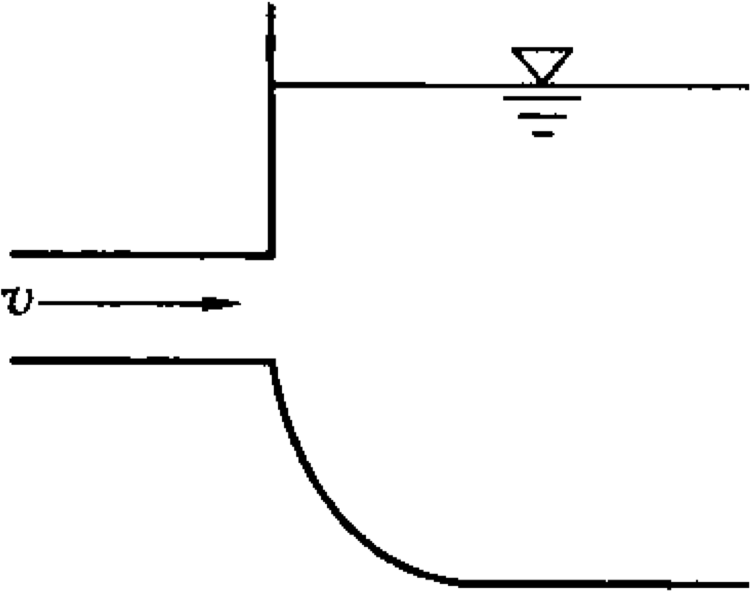
\includegraphics[width=0.72\textwidth,height=0.26\textheight,keepaspectratio]{slides_assets/fluid_deck06/submerged-outflow.png}\\
    {\scriptsize 图：源讲义原图}
  \end{center}
  \TLtakeaway{淹没出流耗散动能；自由出流带出动能。}
\end{frame}

\begin{frame}{E4 突然缩小：经验公式}
  \small
  \TLterm{突然缩小}会在小管入口后形成收缩断面（vena contracta），随后再扩散并掺混，因此也有局部损失。
  \begin{columns}[T]
    \column{0.52\textwidth}
      \textbf{经验公式（适用：突然缩小管）。}
      \[
        h_j=\zeta\frac{v_2^2}{2g},
        \qquad
        \zeta=0.5\left(1-\frac{A_2}{A_1}\right).
        \tag{H37}
      \]
      \begin{itemize}
        \item $v_2$ 是缩小后小管中的平均流速。
        \item 该式是经验式，不像突扩那样有干净的控制体推导。
        \item 定性上，突扩分离区更强；定量比较要先统一速度基准。
      \end{itemize}
    \column{0.48\textwidth}
      \centering
      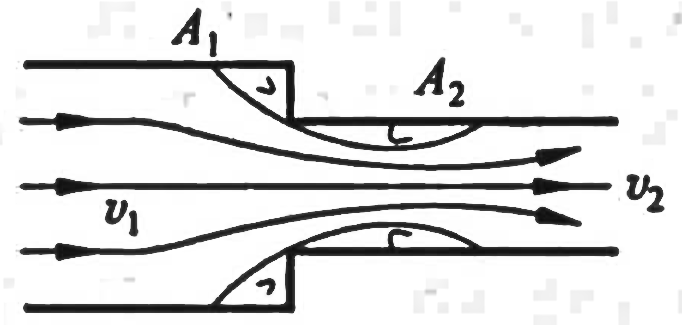
\includegraphics[width=\linewidth,height=0.62\textheight,keepaspectratio]{slides_assets/fluid_deck06/sudden-contraction.png}\\
      {\scriptsize 图：源讲义原图}
  \end{columns}
  \TLtakeaway{突然缩小公式使用小管速度 $v_2$。}
\end{frame}

\begin{frame}{E5 局部损失系数对比}
  \small
  这一节的公式最容易错在速度基准；下表把每个局部构件的公式口径放在同一页。
  \begin{center}
  \footnotesize
  \setlength{\tabcolsep}{3pt}
  \renewcommand{\arraystretch}{1.12}
  \begin{tabular}{@{}p{0.18\textwidth}p{0.16\textwidth}p{0.34\textwidth}p{0.20\textwidth}@{}}
    \toprule
    构件 & 公式性质 & 关键公式 & 速度基准 \\
    \midrule
    突然扩大 & 推导式 &
    $h_j=(v_1-v_2)^2/(2g)$；$\zeta_1=(1-A_1/A_2)^2$；$\zeta_2=(A_2/A_1-1)^2$ &
    可用 $v_1$ 或 $v_2$，但 $\zeta$ 不同 \\
    淹没出流 & 突扩极限 &
    $A_2\gg A_1,\ v_2\approx0$；$h_j=v_1^2/(2g)$；$\zeta=1$ &
    管内出口速度 $v_1$ \\
    自由出流 & 口径说明 &
    出口局部损失通常忽略；动能带出系统 &
    不作为管内局部损失计算 \\
    突然缩小 & 经验式 &
    $h_j=\zeta v_2^2/(2g)$；$\zeta=0.5(1-A_2/A_1)$ &
    缩小后小管速度 $v_2$ \\
    \bottomrule
  \end{tabular}
  \end{center}
  \TLtakeaway{$\zeta$ 必须与对应速度基准一起使用。}
\end{frame}

% =============================================================================
% F. 常见误区
% =============================================================================
\TLsection{常见误区}

\begin{frame}{F1 误区：把 $h_f\propto v^2$ 当成恒真}
  \small
  \TLwarnblock{误区 1：$h_f$ 一定正比 $v^2$}{
    这句话只在\TLterm{阻力平方区}近似成立，因为此时 $\lambda$ 主要由 $\Delta/d$ 决定，可近似看成常数。
  }
  层流中 $\lambda$ 会随速度改变。把 $\Rey=vd/\nu$ 代入 $\lambda=64/\Rey$：
  \[
    h_f
    =
    \frac{64\nu}{vd}\frac{l}{d}\frac{v^2}{2g}
    =
    \frac{32\nu l}{gd^2}\,v .
    \tag{H38}
  \]
  \begin{itemize}
    \item 层流：$h_f\propto v$。
    \item 阻力平方区：$\lambda=f(\Delta/d)$，所以 $h_f\propto v^2$。
  \end{itemize}
  \TLtakeaway{判断速度幂次时，先问 $\lambda$ 是否也随 $v$ 改变。}
\end{frame}

\begin{frame}{F2 误区：$\lambda$ 变小就代表损失变小}
  \small
  \TLwarnblock{误区 2：层流中 $\Rey$ 增大时 $\lambda$ 反而减小，所以 $h_f$ 会减小}{
    层流公式确实给出 $\lambda=64/\Rey$，但达西公式里还有速度水头 $v^2/(2g)$。
  }
  在同一根管、同一种流体中，$\Rey\propto v$，因此
  \[
    \lambda\propto v^{-1},\qquad
    h_f=\lambda\frac{l}{d}\frac{v^2}{2g}\propto v^{-1}v^2=v .
    \tag{H39}
  \]
  \begin{center}
  \footnotesize
  \begin{tabular}{@{}lll@{}}
    \toprule
    量 & 层流中随 $v$ 的趋势 & 净效果 \\
    \midrule
    $\lambda$ & 变小，约为 $v^{-1}$ & 单独看会误导 \\
    $v^2/(2g)$ & 变大，约为 $v^2$ & 主导水头损失增加 \\
    $h_f$ & 变大，约为 $v^1$ & 净指数为 $1$ \\
    \bottomrule
  \end{tabular}
  \end{center}
  \TLtakeaway{不要只看 $\lambda$；沿程损失由 $\lambda$ 与速度水头共同决定。}
\end{frame}

\begin{frame}{F3 误区：曼宁糙率可以随便换单位}
  \small
  \TLwarnblock{误区 3：谢才/曼宁公式只要形式相同，$R$ 用米或英尺都一样}{
    曼宁糙率 $n$ 有量纲。SI 制中 $n$ 的单位是 $\mathrm{m^{-1/3}s}$，所以水力半径 $R$ 必须用米代入。
  }
  曼宁公式
  \[
    v=\frac{1}{n}R^{2/3}i^{1/2},\qquad
    C=\frac{1}{n}R^{1/6}.
    \tag{H40}
  \]
  \begin{itemize}
    \item 若 $R$ 改用 ft，$n$ 的数值也必须换成英制口径。
    \item 只把 $R=1\,\mathrm m$ 改写成 $3.281\,\mathrm{ft}$ 再代入同一个 $n$，会制造量纲错误。
  \end{itemize}
  \TLtakeaway{曼宁公式不是纯无量纲关系；使用表中 $n$ 前必须确认单位制。}
\end{frame}

\begin{frame}{F4 误区：速度基准与“过渡区”混用}
  \small
  \TLwarnblock{误区 4：局部损失中的 $v$ 随便取一个断面速度}{
    $\zeta$ 总是和某个速度水头配套。突然扩大若用小截面速度，则 $v=v_1$，且 $\zeta=(1-A_1/A_2)^2$。
  }
  \TLwarnblock{误区 5：紊流“粗糙过渡区”等于层流到紊流的过渡区}{
    二者不是同一件事：前者是在已经紊流的条件下，粗糙凸起相对粘性底层的作用逐渐增强。
  }
  \begin{center}
  \footnotesize
  \begin{tabular}{@{}lll@{}}
    \toprule
    名称 & 位置 & 含义 \\
    \midrule
    层流到紊流过渡区 & $\Rey$ 约 $2000$--$4000$ & 流态本身不稳定 \\
    紊流粗糙过渡区 & 紊流内部分区 & $\lambda$ 同时受 $\Rey$ 与 $\Delta/d$ 影响 \\
    \bottomrule
  \end{tabular}
  \end{center}
  \TLtakeaway{局部损失先核对速度基准；紊流分区先核对“过渡”指的是流态还是粗糙作用。}
\end{frame}

% =============================================================================
% G. 练习
% =============================================================================
\TLsection{练习}

\begin{frame}{G1 $\star$ 圆管层流 $h_f$}
  \small
  已知圆管直径 $d=0.05\,\mathrm m$，长度 $L=20\,\mathrm m$，运动粘度 $\nu=1.0\times10^{-6}\,\mathrm{m^2/s}$，断面平均流速 $v=0.02\,\mathrm{m/s}$。求 $\Rey$、$\lambda$ 与沿程水头损失 $h_f$。
  \[
    \Rey=\frac{vd}{\nu},\qquad
    h_f=\lambda\frac{L}{d}\frac{v^2}{2g}.
    \tag{H41}
  \]
  \textbf{提示。}
  \begin{enumerate}
    \item 先用 $\Rey=vd/\nu$ 判断流态。
    \item 若为层流，直接用 $\lambda=64/\Rey$。
    \item 最后把 $v^2/(2g)$ 写成 $0.02^2/19.62$。
  \end{enumerate}
  \TLtakeaway{本题训练层流中 $\lambda=64/\Rey$ 与达西公式的直接代入。}
\end{frame}

\begin{frame}{G2 $\star$ 阀门局部损失}
  \small
  某阀门局部损失系数 $\zeta=5.0$，通过阀门的断面平均流速为 $v=2.0\,\mathrm{m/s}$。取 $g=9.81\,\mathrm{m/s^2}$，求局部水头损失 $h_j$。
  \[
    h_j=\zeta\frac{v^2}{2g}.
    \tag{H42}
  \]
  \textbf{提示。}
  \begin{enumerate}
    \item 本题已经给出 $\zeta$，不需要再查表。
    \item 速度水头先算 $v^2/(2g)=4/19.62$。
    \item 结果单位是米水头。
  \end{enumerate}
  \TLtakeaway{局部损失题的第一步永远是确认 $\zeta$ 对应的速度。}
\end{frame}

\begin{frame}{G3 $\star\star$ 紊流光滑管：布拉休斯公式}
  \small
  已知圆管 $d=0.10\,\mathrm m$，$L=50\,\mathrm m$，$v=1.5\,\mathrm{m/s}$，$\nu=1.0\times10^{-6}\,\mathrm{m^2/s}$。按光滑管布拉休斯公式估算 $\lambda$ 与 $h_f$。
  \[
    \lambda=\frac{0.3164}{\Rey^{1/4}},
    \qquad
    h_f=\lambda\frac{L}{d}\frac{v^2}{2g}.
    \tag{H43}
  \]
  \textbf{提示。}
  \begin{enumerate}
    \item 先算 $\Rey=vd/\nu=1.5\times10^5$。
    \item 严格边界常写到 $10^5$，但教材中常把布拉休斯式近似延伸到 $3\times10^5$。
    \item 可用两次开方估计 $\Rey^{1/4}$。
  \end{enumerate}
  \TLtakeaway{本题训练“先判流态，再用经验式查 $\lambda$，最后代入达西公式”。}
\end{frame}

\begin{frame}{G4 $\star\star$ 突然扩大局部损失与 $\zeta$}
  \small
  管道突然扩大：小管 $d_1=0.05\,\mathrm m$，小管速度 $v_1=4\,\mathrm{m/s}$；大管 $d_2=0.10\,\mathrm m$。求扩大后速度 $v_2$、局部损失 $h_j$，以及以 $v_1$ 为基准的 $\zeta$。
  \[
    A_1v_1=A_2v_2,\qquad
    h_j=\frac{(v_1-v_2)^2}{2g},\qquad
    \zeta=\frac{h_j}{v_1^2/(2g)}.
    \tag{H44}
  \]
  \textbf{提示。}
  \begin{enumerate}
    \item 面积比可直接用直径平方比：$A_1/A_2=(d_1/d_2)^2$。
    \item 突然扩大理论式用 $v_1-v_2$。
    \item 用 $v_1$ 作速度水头时，$\zeta=(1-A_1/A_2)^2$ 可作校验。
  \end{enumerate}
  \TLtakeaway{突扩题的关键是把“损失公式”和“速度基准”分开写清楚。}
\end{frame}

\begin{frame}{G5 $\star\star\star$ 柯列布鲁克--怀特迭代}
  \small
  已知圆管 $d=0.20\,\mathrm m$，绝对粗糙度 $\Delta=0.2\,\mathrm{mm}$，$v=2.0\,\mathrm{m/s}$，$\nu=1.0\times10^{-6}\,\mathrm{m^2/s}$。用柯列布鲁克--怀特方程从 $\lambda_0=0.020$ 迭代，取 $L=100\,\mathrm m$ 求 $h_f$。
  \[
    \frac{1}{\sqrt{\lambda}}
    =
    -2\log_{10}
    \left(
      \frac{\Delta}{3.7d}
      +
      \frac{2.51}{\Rey\sqrt{\lambda}}
    \right).
    \tag{H45}
  \]
  \textbf{提示。}
  \begin{enumerate}
    \item 先算 $\Delta/d=0.001$ 与 $\Rey=4.0\times10^5$。
    \item 把右端写成 $-2\log_{10}(2.703\times10^{-4}+6.275\times10^{-6}/\sqrt{\lambda})$。
    \item 迭代两次通常已经收敛到 $\lambda\approx0.0204$。
  \end{enumerate}
  \TLtakeaway{隐式经验式不能直接代入一次结束；要说明初值、迭代式和收敛判断。}
\end{frame}

\begin{frame}{G6 $\star\star\star$ 谢才--曼宁明渠流量}
  \small
  梯形明渠断面：底宽 $b=2\,\mathrm m$，水深 $h=1\,\mathrm m$，边坡 $m=1$，糙率 $n=0.014\,\mathrm{m^{-1/3}s}$，底坡 $i=0.001$。求流速 $v$ 与流量 $Q$。
  \[
    A=(b+mh)h,\qquad
    \chi=b+2h\sqrt{1+m^2},\qquad
    v=\frac{1}{n}R^{2/3}i^{1/2}.
    \tag{H46}
  \]
  \textbf{提示。}
  \begin{enumerate}
    \item 先求过水面积 $A$、湿周 $\chi$ 与水力半径 $R=A/\chi$。
    \item 可先算谢才系数 $C=(1/n)R^{1/6}$，再用 $v=C\sqrt{Ri}$。
    \item 用曼宁直接式 $v=(1/n)R^{2/3}i^{1/2}$ 复核。
  \end{enumerate}
  \TLtakeaway{明渠题的核心不是背公式，而是先把几何量 $A,\chi,R$ 算对。}
\end{frame}

% =============================================================================
% H. 延伸与文献注记
% =============================================================================
\TLsection{延伸与文献注记}

\begin{frame}{H1 历史人物与公式谱系}
  \small
  管流与明渠阻力公式不是一次推导完成的，而是由实验、量纲分析和经验整理逐步拼成。
  \begin{center}
  \footnotesize
  \setlength{\tabcolsep}{3pt}
  \renewcommand{\arraystretch}{1.06}
  \begin{tabular}{@{}p{0.23\textwidth}p{0.18\textwidth}p{0.49\textwidth}@{}}
    \toprule
    人物 & 年代 & 贡献线索 \\
    \midrule
    达西 & 1803--1858 & 渗流与管流实验，为阻力公式提供实验基础 \\
    威斯巴赫 & 1806--1871 & 把管流沿程损失公式化为工程可用形式 \\
    布拉休斯 & 1883--1970 & 给出光滑管紊流经验相关式 \\
    尼古拉兹 & 1894--1979 & 用人工粗糙管实验揭示五个阻力区 \\
    柯列布鲁克与怀特 & 1937--1939 & 整理自然粗糙管的隐式阻力公式 \\
    穆迪 & 1944 & 把 $\lambda$--$\Rey$--$\Delta/d$ 关系绘成穆迪图 \\
    谢才 & 1718--1798 & 提出明渠均匀流经验公式 \\
    曼宁 & 1816--1897 & 用糙率系数 $n$ 估计谢才系数 \\
    \bottomrule
  \end{tabular}
  \end{center}
  \TLtakeaway{本章公式的共同本质是“实验整理 + 能量损失记账”；不要把所有公式都误认为第一性原理推导。}
\end{frame}

\begin{frame}{H2 穆迪图的工程用法}
  \small
  \TLterm{穆迪图}把 $\lambda$ 看成 $\Rey$ 与 $\Delta/d$ 的函数；工程计算时常按“先算 $\Rey$ 与相对粗糙度，再读图或代公式”的流程走。
  \begin{columns}[T]
    \column{0.52\textwidth}
      \textbf{读图步骤。}
      \begin{enumerate}
        \item 计算 $\Rey=vd/\nu$。
        \item 计算相对粗糙度 $\Delta/d$。
        \item 在图上找到对应曲线并读取 $\lambda$。
        \item 代入达西--威斯巴赫公式求 $h_f$。
      \end{enumerate}
    \column{0.48\textwidth}
      若需要显式近似，可用 Swamee--Jain 公式：
      \[
        \lambda
        \approx
        \frac{0.25}
        {\left[
        \log_{10}\!\left(
          \frac{\Delta}{3.7d}
          +
          \frac{5.74}{\Rey^{0.9}}
        \right)\right]^2}.
        \tag{H-empirical-SJ}
      \]
      常见工程范围内误差通常小于 $3\%$。
  \end{columns}
  \TLtakeaway{穆迪图适合手算查表；显式近似适合程序或迭代前的初值估计。}
\end{frame}

\begin{frame}{H3 参考教材与源讲义位置}
  \small
  本讲义把第五章 5.3--5.5 的计算链条写成自学版；进一步学习时可用下列资料交叉核对术语、例题和工程适用范围。
  \begin{center}
  \footnotesize
  \setlength{\tabcolsep}{3pt}
  \renewcommand{\arraystretch}{1.08}
  \begin{tabular}{@{}p{0.30\textwidth}p{0.22\textwidth}p{0.38\textwidth}@{}}
    \toprule
    资料 & 侧重点 & 建议用途 \\
    \midrule
    闻德荪《流体力学》 & 中文课程主线 & 对齐本课程符号和中文术语 \\
    吴持恭《水力学》（第四版） & 明渠与水力学工程 & 查谢才、曼宁和局部损失表述 \\
    White, \emph{Fluid Mechanics}, 9th ed. & 工程流体力学 & 对比 Darcy friction factor 与 Moody chart \\
    Munson, \emph{Fundamentals of Fluid Mechanics} & 基础例题 & 复算管流、局部损失与明渠算例 \\
    源讲义第五章 5.3--5.5 节 & 课程依据 & 对照本 deck 的章节顺序与公式编号 \\
    \bottomrule
  \end{tabular}
  \end{center}
  \TLtakeaway{先用本讲义完成自洽计算，再用教材查适用范围、实验背景和更多构件系数。}
\end{frame}

\begin{frame}{H4 全六册回顾}
  \small
  本讲义是本套流体力学自学 deck 的第 6 部分；它把前面建立的“物性、静力、运动、动力、一元恒定流”接到真实流动损失上。
  \begin{center}
  \begin{tikzpicture}[scale=0.70,>={Stealth[length=5pt]}]
    \node[draw=TLprimary,fill=TLprimaryTint,rounded corners=2pt,minimum width=2.6cm,minimum height=0.66cm] (c1) at (-4.9,0.75) {Ch1 流体性质};
    \node[draw=TLprimary,fill=TLprimaryTint,rounded corners=2pt,minimum width=2.6cm,minimum height=0.66cm] (c2) at (-2.9,0.75) {Ch2 静力学};
    \node[draw=TLprimary,fill=TLprimaryTint,rounded corners=2pt,minimum width=2.6cm,minimum height=0.66cm] (c3) at (-0.9,0.75) {Ch3 运动学};
    \node[draw=TLprimary,fill=TLprimaryTint,rounded corners=2pt,minimum width=2.6cm,minimum height=0.66cm] (c4) at (1.1,0.75) {Ch4 动力学};
    \node[draw=TLprimary,fill=TLprimaryTint,rounded corners=2pt,minimum width=2.6cm,minimum height=0.66cm] (c5) at (3.1,0.75) {Ch5 一元流};
    \node[draw=TLaccent,fill=TLaccentLight,rounded corners=2pt,minimum width=2.6cm,minimum height=0.66cm] (c6) at (5.1,0.75) {Ch6 损失};
    \draw[->,TLprimaryDark,thick] (c1)--(c2);
    \draw[->,TLprimaryDark,thick] (c2)--(c3);
    \draw[->,TLprimaryDark,thick] (c3)--(c4);
    \draw[->,TLprimaryDark,thick] (c4)--(c5);
    \draw[->,TLprimaryDark,thick] (c5)--(c6);
    \node[align=center,TLinkSoft,text width=11cm] at (0,-0.55)
      {流体性质 $\to$ 静力学 $\to$ 运动学 $\to$ 动力学方程 $\to$ 一元恒定流 $\to$ 紊流与损失。};
  \end{tikzpicture}
  \end{center}
  \begin{itemize}
    \item 前五册给出“无损或理想化”的守恒框架。
    \item 本册把粘性、粗糙度、局部构件和明渠经验公式放回工程计算。
  \end{itemize}
  \TLtakeaway{真实流动计算的闭环是：守恒方程给骨架，损失公式给工程闭合。}
\end{frame}

% =============================================================================
% I. 术语速查
% =============================================================================
\TLsection{术语速查}

\begin{frame}{术语速查（一）：损失与阻力系数}
  \begin{center}
  \vspace{4pt}
  \footnotesize
  \setlength{\tabcolsep}{3pt}
  \renewcommand{\arraystretch}{1.08}
  \begin{tabular}{@{}lll@{}}
    \toprule
    中文术语 & English Term & 符号/说明 \\
    \midrule
    沿程水头损失 & \shortstack[l]{major (frictional)\\head loss} & $h_f$ \\
    局部水头损失 & \shortstack[l]{minor (local)\\head loss} & $h_j$ \\
    沿程损失系数 & Darcy friction factor & $\lambda$，穆迪图使用 \\
    达西--威斯巴赫公式 & \shortstack[l]{Darcy--Weisbach\\equation} & $h_f=\lambda(l/d)(v^2/2g)$ \\
    水力坡度 & hydraulic gradient & $J=h_f/l$ \\
    雷诺数 & Reynolds number & $\Rey=vd/\nu$ \\
    阻力平方区 & \shortstack[l]{fully rough\\turbulent regime} & $\lambda=f(\Delta/d)$ only \\
    \bottomrule
  \end{tabular}
  \end{center}
  \TLtakeaway{第一组术语回答“损失怎样命名、$\lambda$ 和 $\Rey$ 怎样进入达西公式”。}
\end{frame}

\begin{frame}{术语速查（二）：明渠、局部损失与图表}
  \begin{center}
  \vspace{4pt}
  \footnotesize
  \setlength{\tabcolsep}{3pt}
  \renewcommand{\arraystretch}{1.08}
  \begin{tabular}{@{}lll@{}}
    \toprule
    中文术语 & English Term & 符号/说明 \\
    \midrule
    谢才系数 & Chézy coefficient & $C\,[\mathrm{m^{1/2}/s}]$ \\
    糙率 & \shortstack[l]{Manning roughness\\coefficient} & $n\,[\mathrm{m^{-1/3}s}]$ \\
    局部损失系数 & \shortstack[l]{loss (minor loss)\\coefficient} & $\zeta$ \\
    柯列布鲁克--怀特方程 & \shortstack[l]{Colebrook--White\\equation} & implicit $\lambda$ \\
    穆迪图 & Moody chart & $\lambda$ vs. $\Rey,\Delta/d$ \\
    布拉休斯相关式 & Blasius correlation & $\lambda=0.3164/\Rey^{1/4}$ \\
    \bottomrule
  \end{tabular}
  \end{center}
  \TLtakeaway{第二组术语回答“明渠经验公式、局部构件系数和紊流查图怎样命名”。}
\end{frame}

\appendix
\TLsection{附录：习题解答}

\begin{frame}{附录 G1 解答}
  \footnotesize
  先判断流态：
  \[
    \Rey=\frac{vd}{\nu}
    =
    \frac{0.02\times0.05}{1.0\times10^{-6}}
    =
    1000 .
    \tag{H47}
  \]
  因为 $\Rey=1000<2000$，该流动为层流，所以
  \[
    \lambda=\frac{64}{\Rey}
    =
    \frac{64}{1000}
    =
    0.064 .
    \tag{H48}
  \]
  代入达西--威斯巴赫公式：
  \[
    h_f
    =
    0.064\times\frac{20}{0.05}\times\frac{0.02^2}{19.62}
    =
    0.064\times400\times2.039\times10^{-5}
    =
    5.22\times10^{-4}\,\mathrm m .
    \tag{H49}
  \]
  \TLresultblock{答案}{
    \[
      \boxed{\Rey=1000,\quad \lambda=0.064,\quad h_f\approx5.2\times10^{-4}\,\mathrm m.}
    \]
  }
\end{frame}

\begin{frame}{附录 G2 解答}
  \footnotesize
  阀门局部损失直接代入局部损失公式：
  \[
    h_j
    =
    \zeta\frac{v^2}{2g}
    =
    5.0\times\frac{2.0^2}{2\times9.81}
    =
    \frac{20}{19.62}
    =
    1.019\,\mathrm m .
    \tag{H50}
  \]
  这里的 $v$ 是题面给出的阀门所在截面平均流速；如果表格中的 $\zeta$ 改用别的速度基准，必须同步更换。
  \TLresultblock{答案}{
    \[
      \boxed{h_j\approx1.02\,\mathrm m.}
    \]
  }
\end{frame}

\begin{frame}{附录 G3 解答}
  \footnotesize
  先计算雷诺数：
  \[
    \Rey
    =
    \frac{vd}{\nu}
    =
    \frac{1.5\times0.10}{1.0\times10^{-6}}
    =
    150000 .
    \tag{H51}
  \]
  题面指定使用布拉休斯公式；四次方根用两次开方估计：
  \[
    150000^{1/4}
    =
    \sqrt{\sqrt{150000}}
    \approx
    \sqrt{387.3}
    \approx
    19.68,\qquad
    \lambda=\frac{0.3164}{19.68}=0.01608 .
    \tag{H52}
  \]
  代入达西公式：
  \[
    h_f
    =
    0.0161\times\frac{50}{0.10}\times\frac{1.5^2}{19.62}
    =
    0.0161\times500\times0.1147
    =
    0.923\,\mathrm m .
    \tag{H53}
  \]
  \TLresultblock{答案}{
    \[
      \boxed{\Rey=1.5\times10^5,\quad \lambda\approx0.0161,\quad h_f\approx0.92\,\mathrm m.}
    \]
  }
\end{frame}

\begin{frame}{附录 G4 解答}
  \footnotesize
  两个圆管面积分别为
  \[
    A_1=\frac{\pi(0.05)^2}{4}=1.963\times10^{-3}\,\mathrm{m^2},
    \qquad
    A_2=\frac{\pi(0.10)^2}{4}=7.854\times10^{-3}\,\mathrm{m^2}.
    \tag{H54}
  \]
  连续方程给出扩大后速度：
  \[
    v_2
    =
    v_1\frac{A_1}{A_2}
    =
    4\times\frac{1.963\times10^{-3}}{7.854\times10^{-3}}
    =
    1.0\,\mathrm{m/s}.
    \tag{H55}
  \]
  突然扩大损失为
  \[
    h_j=\frac{(v_1-v_2)^2}{2g}
    =
    \frac{(4-1)^2}{19.62}
    =
    0.459\,\mathrm m .
    \tag{H56}
  \]
  以 $v_1$ 为基准的局部损失系数为
  \[
    \zeta
    =
    \frac{h_j}{v_1^2/(2g)}
    =
    \frac{0.459}{16/19.62}
    =
    0.563\approx0.56.
    \tag{H57}
  \]
  \TLresultblock{答案}{
    \[
      \boxed{v_2=1.0\,\mathrm{m/s},\quad h_j\approx0.46\,\mathrm m,\quad \zeta\approx0.56.}
    \]
  }
\end{frame}

\begin{frame}{附录 G5 解答}
  \footnotesize
  \setlength{\abovedisplayskip}{3pt}
  \setlength{\belowdisplayskip}{3pt}
  先计算两个无量纲输入：
  \[
    \frac{\Delta}{d}=\frac{0.0002}{0.20}=0.001,\qquad
    \Rey=\frac{2.0\times0.20}{1.0\times10^{-6}}=400000.
    \tag{H58}
  \]
  柯列布鲁克--怀特方程化为本题的迭代式：
  \[
    \frac{1}{\sqrt{\lambda}}
    =
    -2\log_{10}
    \left(2.703\times10^{-4}
    +
    \frac{6.275\times10^{-6}}{\sqrt{\lambda}}\right).
    \tag{H59}
  \]
  从 $\lambda_0=0.020$ 开始：
  \[
    \sqrt{\lambda_0}=0.1414,\quad
    \text{arg}=2.703\times10^{-4}+4.437\times10^{-5}=3.147\times10^{-4},
    \quad
    \lambda_1=\frac{1}{7.003^2}=0.02038 .
    \tag{H60}
  \]
  第二次迭代：
  \[
    \sqrt{\lambda_1}=0.1428,\quad
    \text{arg}=2.703\times10^{-4}+4.394\times10^{-5}=3.142\times10^{-4},
    \quad
    \lambda_2\approx0.0204 .
    \tag{H61}
  \]
  因此
  \[
    h_f
    =
    0.0204\times\frac{100}{0.20}\times\frac{2.0^2}{19.62}
    =
    0.0204\times500\times0.2039
    =
    \boxed{2.08\,\mathrm m}.
    \tag{H62}
  \]
\end{frame}

\begin{frame}{附录 G6 解答}
  \footnotesize
  \setlength{\abovedisplayskip}{3pt}
  \setlength{\belowdisplayskip}{3pt}
  梯形断面的面积、湿周和水力半径为
  \[
    A=(b+mh)h=(2+1\times1)\times1=3\,\mathrm{m^2},
    \quad
    \chi=2+2\sqrt2=4.828\,\mathrm m,
    \quad
    R=\frac{3}{4.828}=0.6215\,\mathrm m .
    \tag{H63}
  \]
  先按谢才--曼宁关系求谢才系数：
  \[
    R^{1/6}
    =
    \exp\!\left(\frac{\ln0.6215}{6}\right)
    =
    \exp(-0.07937)
    =
    0.9237,\qquad
    C=\frac{1}{0.014}\times0.9237=65.98 .
    \tag{H64}
  \]
  因而
  \[
    v=C\sqrt{Ri}
    =
    66.0\sqrt{0.6215\times0.001}
    =
    66.0\times0.02493
    =
    1.645\,\mathrm{m/s},
    \qquad
    Q=Av=3\times1.645=4.93\,\mathrm{m^3/s}.
    \tag{H65}
  \]
  用曼宁直接式复核：
  \[
    R^{2/3}
    =
    \exp\!\left(\frac{2}{3}\ln0.6215\right)
    =
    0.7281,\qquad
    v=\frac{1}{0.014}\times0.7281\times\sqrt{0.001}
    =
    1.645\,\mathrm{m/s}.
    \tag{H66}
  \]
  \[
    \boxed{v\approx1.65\,\mathrm{m/s},\qquad Q\approx4.93\,\mathrm{m^3/s}.}
  \]
\end{frame}

\end{document}
